\documentclass[12pt,oneside]{book}
\include{macros/style}

% Long Table and decimal aligned columns
\usepackage{dcolumn}
\usepackage{longtable}
\usepackage{multicol}
\usepackage{multirow}

% Mathematics support
\usepackage{amsmath}
\usepackage{amsthm}
\usepackage{amssymb}


% Text Control
\usepackage{xspace}
\usepackage{textcase}

% Graphics
\usepackage{wasysym}
\usepackage{graphics}
\usepackage{graphicx}   % A package to allow insertion of
                        % external image files

\usepackage{listings}
\usepackage{float}
\usepackage{placeins}
\usepackage{longtable} % <---- new
\usepackage{fancyhdr,graphicx,amsmath,amssymb}
\usepackage{fullpage}
\usepackage{times}
\usepackage{float}
\usepackage{xr}
\usepackage{caption}
\usepackage{xcolor}
\usepackage[linesnumbered,ruled,vlined]{algorithm2e}
\SetKwRepeat{Struct}{struct \{}{\}}%
\SetKwRepeat{Union}{union \{}{\}}%
\newcommand\mycommfont[1]{\footnotesize\ttfamily\textcolor{blue}{#1}}
\SetCommentSty{mycommfont}
\usepackage{listings}
\lstset{
  basicstyle=\ttfamily,
  columns=fullflexible,
  frame=single,
  breaklines=true,
  postbreak=\mbox{\textcolor{red}{$\hookrightarrow$}\space},
}
\begin{document}

% Front Matter
\input frontmatter/fm

\newpage

	\startfirstchapter{Introduction}
\label{chapter:introduction}
Vulnerabilities in software enable the exploitation of the computer or system they are running on. Therefore, the emphasis placed on computer security particularly in the field of software vulnerabilities has increased dramatically. It's important for software developers to build secure applications. Unfortunately, building secure software is expensive. Vendors usually comply with their own quality assurance measures which focus on marketable concerns while leaving security to a lower priority or even worse, they totally ignore it. Therefore, fully relying on the vendor of the software to secure your system and data is impractical and risky. \cite{dowd_art_2006}

Software security review conducted by a third party is neccessary. One approach of software security review is software auditing. It is a process of analyzing the software in the forms of source code or binary. This auditing can uncover some hard to reveal vulnerabilities which might be exploited by hackers. Identification of these security holes can save users of the software from putting their sensitive data and business resources at risk. \cite{dowd_art_2006}

Most of the software vulnerabilities are stimulated by malicious data, and it is valuable to understand how this malicious data triggers the unexpected behaviors of the system. In most cases, this malicious data is injected by attackers into the system to trigger the exploitation. In some complex systems, several programs work together to provide a service or functionality. In these situations, the malicious data might have passed through multiple components of the system and be modified before it reaches the vulnerable point and ultimately triggers an exploitable condition of the system. As a consequence, the flow of data throughout the system's different programs is considered to be one of the most important aspects to analyze during a security review. \cite{dowd_art_2006}

The data flow among various programs within a system or across different systems helps to understand how the system works, as well as potentially disclose the vulnerabilities in a system. There are multiple mechanisms to grab the data across programs, and the methods for obtaining this data flow can affect the analysis results greatly. 

In this research, I develop a method to identify communications between programs by analysing assembly level execution traces. This method can guide security engineers to investigate the communications of the programs in the circumstance that they have the captured execution traces and want to understand the interaction behaviour of the programs. The research is not specific for vulnerabilities detection but generalized for the comprehension of the interacting behaviour of two programs.

\section{Motivation}
This project started with an informal requirement from our research partner DRDC (Defence Research and Development Canada). for visualizing multiple assembly traces to assist their software and security analysis. The literature review and conversations with DRDC help to clarify the goal and guided this research. In this section, I discuss the need for performing assembly trace investigation for communication analysis. First I explain why security engineers perform assembly trace analysis. Then I elaborate why they need to perform communication analysis at the assembly trace level. 

\subsection{Why Assembly Trace Analysis}
Dynamic analysis of programs is adopted mainly in software maintenance and security auditing \cite{zhang2010detecting}, \cite{cai2016sworddta}, \cite{somorovsky2016systematic}. Sanjay Bhansali et al. claim that program execution traces with the most intimate detail of a program's dynamic behavior can facilitate program optimization and failure diagnosis. Jonas Tr{\"u}mper et al. give a example of how tracing can facilitate software-maintenance tasks \cite{trumper2012maintenance}.

Dynamic analysis can be done using debuggers, however, debuggers would halt the execution of the system and result in a distortion of the timing behavior of the running system \cite{trumper2012maintenance}. Instead, tracing a running program with instrumentation would provide more accurate run time behaviour information about the system. 

The instrumentation of the tracing can be done at various levels of granularity, such as programming language or machine language instructions. The access to a software can be divided into five categories, with variations: source only, binary only, both source and binary access, checked build, strict black box. Only having the binary is common when performing vulnerability research on closed-source commercial software\cite{dowd_art_2006}. In this case, assembly level tracing is the only option to do a security review of the software.

On the other hand, the binary code is what is running on the system, binary tracing is more representative for software security engineers than the source code in the terms of auditing. Some bugs might appear because of a compilation problem or because the compiler optimized some code that is necessary to make the system secure. The piece of code listed below is an example in which the line of code resetting the password before the program end would be optimized by the compliers if they implement the dead store elimination\cite{howard2003writing}. For example, with the -fdse option, the GNU Compiler Collection(GCC) will perform the dead store elimination and -fdse is enabled by default at -O and higher optimization level \cite{gcc}. This will make the user's password stay in memory, which is considered as potential security risk. However, looking at the source code does not reveal the problem.

\begin{lstlisting}[language=C++, caption= Password Fetching Example ]
#include <iostream>
#include <string>
#include <conio.h>
using namespace std;
int main(){
   string password ="";
   char ch;
   cout << "Enter password";
   ch = _getch();
   while(ch != 13){//character 13 is enter
      password.push_back(ch);
      cout << '*';
      ch = _getch();
   }   
   if(checkPass(password)){
     allowLogin();
   }  
   password ="";
}
\end{lstlisting}

\subsection{Why Communication Analysis with Assembly Traces}
Programs nowadays do not always work in isolation. The communication and interaction between programs affects the behaviour of the system. Without knowing how a program works with others, an analysis of the isolated execution trace on a single computer is usually futile. Data flow tracing between programs is essential to review both the design and implementation of the software.

Many network sniffers, such as Wireshark\cite{_wireshark_????} and Tcpdump\cite{tcpdump_tcpdump/libpcap_????}, can help to capture the data flow across the network. However, this method  is insufficient because security problems can occur even if the information sent is correct. Therefore, analysing the communications with transmitted data in instruction and memory access level is a solid way to evaluate the security of a system.

Shameng Wen et al. argue that fuzz testing and symbolic execution are widely applied to detect vulnerabilities in network protocol implementations. Their work focuses on designing a model which guides the symbolic execution for fuzz testing \cite{wen2017model} but ignores the analysis of the output, the execution traces. Furthermore, their work focused only on the network protocol implementation and is not generalized to all communications.

Besides vulnerabilities detection and security analysis, communication analysis with assembly traces can also be a way to learn how the work is performed by the system or validate a specification of it. Our research partner DRDC provided some use cases in which they require the assistance of communication analysis to understand their systems. The first one is related to their work with embedded systems. These systems often have more than one processor, each specialized for a specific task, that coordinate to complete the overall job of that device.  In another case, the embedded device will work with a normal computer and exchange information with it through some means
(USB, wireless, etc.).  For instance, the data might be coming in from an external sensor in an analog form, transformed by a Digital Signal Processor (DSP) in a device, sent to a more generic processor inside that device to integrate with other data, then sent wirelessly to an external computer. Being able to visualize more than one trace would help them follow the flow of data through the system at the same time that they trace the execution of the programs.

Overall, communication analysis with assembly traces is a way to learn how the work is performed by the system. 

\section{Research Goal}
The goal of this research is to design a method for communication analysis using the execution traces of the interacting programs. This method should be general enough for all message based communication analysis between programs regardless of their programming language, host operating system or selected execution tracer. 

\section{Research Process}
Figure \ref{methodology} shows the overview of my iterative research process with three abstracted stages. The process is iterative because the implementation changed several times due to changes with the model, and the model was modified based on understanding of details of execution traces gained throughout the implementation. 

\begin{figure}[H]
  \centerline{\includegraphics[scale=0.44]{Figures/methodology}}
  \caption{Research Approach overview}
  \label{methodology}
  \end{figure}

This research requires background knowledge of software security and vulnerabilities. I acquired the background knowledge basically from literature review. It helped me acquire the essential concepts of software vulnerabilities and their categories, understand some facilities for vulnerabilities detection and software maintenance in the perspective of security. After that, I was convinced that communication analysis in assembly trace level would benefit software security engineers to understand the behaviour of software and detect software vulnerabilities. 

In order to analyze the communication of programs, I had to know how the communication works. For this purpose, I started the investigation by writing example simple programs with the Windows API and run them locally in my desktop. By understanding their behaviour and reading the Windows API documentation, I abstracted the communication model which is not operating system specific.

The abstract assembly trace definition was built on the generalization of the trace format provided by our research partner, DRDC. I don't have the access to their home-made assembly tracer which is based on PIN\cite{_pin_????}. Fortunately, they provideed me with a comprehensive document about the format of the captured trace and example traces. With these, I grasped the constructive view of the assembly execution trace. Furthermore, some other tools can also capture the required information in assembly level for communication analysis. This supports the generalization of the trace definition and the abstraction of the dual\_trace.

The implementation of the prototype and the communication analysis algorithms were developed in parallel. The high level communication identification algorithm and the specific algorithms for named pipe communication methods were abstracted based on the implementation, while the others are developed theoretically. Two experiments are designed to test this analysis method, the prototype and some algorithms. 


\section{Contributions}
The main contributions of this work can be summarized as:
\begin{itemize}
  \item \textbf{Communication Model:} The communication model in this thesis is an abstract model of the communications between two programs. It was abstracted from the understanding of several communication methods and is general for other communication methods that are not mentioned in this thesis.
  \item \textbf{Dual\_trace Formalization:} By understanding the assembly level execution traces, a dual\_trace was formalized to describe the information that was needed for communication analysis. This model doesn't specify the format of the execution traces but defines what information is necessary to fulfil the analysis requirement. All execution traces that comply with this formalization can be used for the analysis.
  \item \textbf{Communication Analysis Approach:} The overall approach to identify the communications in the dual\_trace is designed. Eight algorithms were developed for the steps in this
approach regarding some communication methods or communication types.
  \item \textbf{Prototype:} A prototype is designed and implemented on Atlantis, which is a assembly execution traces analysis environment \cite{huang2017atlantis}. This prototype demonstrates that the communication analysis approach is feasible. It is a unique tool for the security engineers to analyze the communications of programs via assembly execution trace analysis.
\end{itemize}

\section{Thesis Organization}
In Chapter 2, I summarize the related background information and knowledge needed to understand or related to this work including security and vulnerability, program communication mechanisms, program execution trace tools, and Atlantis. 

Chapter 3 describes the model of the communication between two programs. This model defines the communication in the context of trace analysis and discusses the properties of the communications. 

In Chapter 4, I first present the abstract dual\_trace formulation. Based on this formulation, I describe the communication analysis process and the essential algorithms.

In Chapter 5, I present the implementation of a dual\_trace communication analysis prototype. 

In Chapter 6, I present two experiments of communication analysis with dual\_traces using the implemented prototype. Notably, the results show the communications are correctly identified. 

Finally, in Chapter 7, I conclude the result of this research and outline possible future work.
	\startchapter{Background}
\label{chapter:Bac}
This section introduces several background knowledge or information that related to this work. First I describe what is software security and how important it is as well as our previous approach to assist detection of software vulnerabilities by assembly level trace analysis. Second, I introduce the general assembly level trace as well as some tracer to generate it. Third, I discuss how software interaction affect the behavior of the software and how they related to the software vulnerabilities. Then I talk about Windows Communication Foundation in which the communication channels type used are targeted by this work. Finally, we mention some important Windows function calling conventions without which you can not picture what the function calls look like in the assembly level.
\section{Software Security}
The internet grows incredibly fast in the past few year. More and more computers are connected to it in order to get service or provide service. The internet as a powerful platform for people to share resource, meanwhile, introduces the risk to computers in the way that it enable the exploit of the vulnerabilities of the software running on it. Accordingly, the emphasize placed on computer security particularly in the field of software vulnerabilities detection increases dramatically. It's important for software developers to build secure applications. Unfortunetely, this is usually very expensive and time consuming and somehow impossible. On the other hand, finding issues in the built applications is more important and practical. Howerver this is a complex process and require deep technical understanding in the perspetive of reverse engineering.\cite{dowd_art_2006}.


\section{Software Vulnerability Detection}
A common approach to detect existing vulnerabilities is fuzzing testing, which record the execution trace while supplying the program with input data up to the crash and perform the analysis of the trace to find the root cause of the crash and decide if that is a vulnerability\cite{cleary_reconstructing_2013}. Execution trace can be captured in different levels, for example object level and function level. But my research only focus on those that captured in instruction and memory reference level. There are two main reasons for analysis system-level traces. First, it is for analysis of the software provided by vendor whose source code are not available. The second one is that low level trace are more accurately reflect the instructions that are executed by multicore hardware\cite{wang_predicting_2011}. 


\section{Assembly Level Trace}
There are many tools that can trace a running program in assembly instruction level.  IDA pro \cite{eagle_ida_2008} is a widely used tool in reverse engineering which can capture and analysis system level execution trace. Giving open plugin APIs, IDA pro allows plugin such as Codemap \cite{_c0demap/codemap:_????} to provide more sufficient features for "run-trace" visualization. PIN\cite{_pin_????} as a tool for instrumentation of programs, provides a rich API which allows users to implement their own tool for instruction trace and memory reference trace. Other tools like Dynamic \ref{brueningqz} and 
\section{Software Interaction}
Applications nowaday do not alway work isolately,  many software  appear as  reticula collaborating systems connecting different modules in the network\cite{PhysRevE.68.046116} which make the discovery of vulnerabilities even harder. The communication and interaction between modules affect the behaviour of the software. Without regarding to the synergy information , analysis of the isolated execution trace on a single computer is usually futile. 

\section{Atlantis}
Applications nowaday do not alway work isolately,  many software  appear as  reticula collaborating systems connecting different modules in the network\cite{PhysRevE.68.046116} which make the discovery of vulnerabilities even harder. The communication and interaction between modules affect the behaviour of the software. Without regarding to the synergy information , analysis of the isolated execution trace on a single computer is usually futile. 

\section{Windows Communication Foundation}
We limited our research only on the communication types used in Windows Communication Foundation(WCF) for now. Windows Communication Foundation (WCF) is a framework for building service-oriented applications. Using WCF, developers can send data as asynchronous or asynchronous messages from one service endpoint to another. We are not going deep into the details of this framework but only mention the most common communication methods it supports in its messaging layer. The messaging layer in WCF is composed of channels. A channel is a component that processes a message in some protocol. There are two types of channels in WCF: transport channels and protocol channels. In this work we only care about transport channels. Transport channels read and write messages from the network. Examples of transports are named pipes, MSMQ, TCP/UDP or HTTP, all of which are involved in the scope of this work.


    \externaldocument{../appendix/chapter_app}
\startchapter{Modeling}
\label{chapter:Mod}
In this chapter, I modeled the communication of two running programs. The dual-trace captured from two interacting programs are also modeled in the perspective of communication analysis. The modeling are based on the investigation of some common used communication methods. The communication methods are divided into two categories based on their data transmission properties. This modeling are the foundation to decide how communications being identified from the dual-trace and how to present them to the user. The terminology of using in this chapter can be found in \ref{term}.

\section{Communication Categorization and Communication Methods}
The goal of this work is to identify the communications from the dual-trace. We need to understand the properties of the communications to identify them. In general, there are two types of communication: reliable and unreliable in the terms of their reliability of data transmission. The reason to divide the communication methods into these two categories is that the data transmission properties of the communications fall in different categories affect the mechanism of the data verification in the identification algorithm. In the following two subsections, I summarize the characteristics of these two communication categories. The communication methods list in Table\ref{methodsInCategories} will be discussed further to provide more concrete comprehension. 
\begin{table}[H]
\centering
\caption{Communication Methods Discussed in This Work}
\label{methodsInCategories}
\begin{tabular}{|l|l|}
 \hline
\textbf{Reliable Communication}& \textbf{Unreliable Communication}\\
 \hline
Named Pipes & Message Queue   \\
TCP &  UDP \\
 \hline
\end{tabular}
\end{table}


\subsection{Reliable Communication}\label{reliable}
A reliable communication guarantees the data being sent by one endpoint of the channel always received losslessly and in order to the other endpoint. For some communication methods, a channel can be closed without waiting the completion of all data transmission. With this property, the concatenated data in the receive stream of one endpoint should be the sub string of the concatenated data in the send stream of the other endpoint. Therefore, the send and receive data verification should be in send and receive stream level by comparing the concatenated received data of one endpoint to the concatenated sent data of another. 

\subsection{Unreliable Communication}\label{unreliable}
An unreliable communication does not guarantee the data being sent always arrive the receiver. Moreover, the data packets can arrive to the receiver in any order. However, the bright side of unreliable communication is that the packets being sent are always arrived as the origin packet, no data re-segmentation would happen. Accordingly, the send and receive data verification should be done by matching the data packets in a receive event to a send event on the other side.

\subsection{Communication Methods}
In this section, I describe the mechanism and the basic data transfer characteristics of each communication method in Table\ref{methodsInCategories} briefly. Moreover, data transfer scenarios are represented correspondingly in diagrams for each communication method. 
 
\subsubsection{Named Pipe}
A named pipe provides FIFO communication mechanism for inter-process communication. It can be one-way or duplex pipe which allows two programs send and receive message through the named pipe. \cite{khambattinamed}

The basic data transfer characteristics of Named Pipe are:
\begin{itemize}
  \item Bytes received in order
  \item Bytes sent as a whole trunk can be received in segments
  \item No data duplication
  \item Only the last trunk can be lost
\end{itemize}

Based on these characteristics, the data transfer scenarios of Named pipe can be summarized in Figure\ref{namedpipe}. 
\begin{figure}[H]
\centerline{\includegraphics[scale=0.48]{Figures/namedpipe}}
\caption{Data Transfer Scenarios for Named Pipe}
\label{namedpipe}
\end{figure}

\subsubsection{Message Queue}
Message Queuing (MSMQ) is a communication method to allow applications which are running at different times across heterogeneous networks and systems that may be temporarily offline can still communicate with each other. Messages are sent to and read from queues by applications. Multiple sending applications can send messages to and multiple receiving applications can read messages from one queue.\cite{redkar2004pro} In this work, only one sending application versus one receiving application case is considered. Multiple senders to multiple receivers scenario can be divided into multiple sender and receiver situation. Both applications of a communication can send to and receive from the channel.

The basic data transfer characteristics of Message Queue are:
\begin{itemize}
  \item Bytes sent in packet and received in packet, no bytes re-segmented
  \item Packets can lost
  \item Packets received in order
  \item No data duplication
\end{itemize}
Based on these characteristics, the data transfer scenarios of Message Queue can be summarized in Figure\ref{msmq}.
\begin{figure}[H]
\centerline{\includegraphics[scale=0.48]{Figures/msmq}}
\caption{Data Transfer Scenarios for Message Queue}
\label{msmq}
\end{figure}

\subsubsection{TCP}
TCP is the most fundamental reliable transport method in computer networking. TCP provides reliable, ordered, and error-checked delivery of a stream of octets between applications running on hosts in an IP network. The TCP header contains the sequence number of the sending octets and the acknowledge sequence this endpoint is expecting from the other endpoint(if ACK is set). The re-transmission mechanism is based on the ACK. 

The basic data transfer characteristics of TCP are:
\begin{itemize}
  \item Bytes received in order
  \item No data lost(lost data will be re-transmitted)
  \item No data duplication
  \item Sender window size is different from receiver's window size, so packets can be re-segmented
\end{itemize}

Based on these characteristics,  the data transfer scenarios of TCP can be summarized in Figure\ref{tcp}.
\begin{figure}[H]
\centerline{\includegraphics[scale=0.48]{Figures/tcp}}
 \caption{Data Transfer Scenarios for TCP}
\label{tcp}
\end{figure}

\subsubsection{UDP}
UDP is a widely used unreliable transmission method in computer networking. It is a simple protocol mechanism, which has no guarantee of delivery, ordering, or duplicate protection. This transmission method is suitable for many real time systems. 

The basic data transfer characteristics of UDP are:
\begin{itemize}
  \item Bytes sent in packet and received in packet, no re-segmentation
  \item Packets can lost
  \item Packets can be duplicated
  \item Packets can arrive receiver out of order
\end{itemize}

Based on these characteristics, the data transfer scenarios of UDP can be summarized in Figure\ref{upd}.
\begin{figure}[H]
\centerline{\includegraphics[scale=0.48]{Figures/udp}}
 \caption{Data Transfer Scenarios for UDP}
\label{upd}
\end{figure}

\section{Communication Model}\label{definition}
The communication of two programs is defined in this section. The communication in this work is data transfer activities between two running programs through a specific channel. Some collaborative activities between the programs such as remote procedure call is out of the scope of this research. Communication among multiple programs (more than two) is not discussed in this work. The channel can be reopened again to start new communications after being closed. However, the reopened channel will be treated as a new communication. The way that I define the communication is leading to the communication identification in the dual-trace. So the definition is not about how the communication works but what it looks like. There are many communication methods in the real world and they are compatible to this communication definition. 

A communication $Co$ is defined by the 2-tuple $\langle ep, c \rangle$, where $ep$ is a set $\left\lbrace e_{x}: x= 0,1\right\rbrace $ for the two endpoints communicating with each other though the channel $c$ which represented by a identifier. The endpoint $e_{x}$ is defined by the 3-tuple $\langle h_{x}, ds_{x}, dr_{x}\rangle$. $h_{x}$ is the handle created within a process for subsequent data transfer operations. $ds_{x}$ is the sequence of packets sent in the sending operations of $h_{x}$ while $dr_{x}$ is the sequence of packets received in the receiving operations of $h_{x}$. $e_{0}$ is created in process $p$ and $e_{1}$ is created in process $q$. Let $ds_{x} = \left(ps_{x,i}: 0\leqslant i \leqslant I_{x} \right)$ and $dr_{x} = \left(pr_{x,j}: 0\leqslant j \leqslant J_{x} \right)$ in which $ps_{x,i} = \langle ts_{x,i}, ss_{x,i} \rangle$ and $pr_{x,i} = \langle tr_{x,j}, sr_{x,j} \rangle$. $ts_{x,i}$ and $tr_{x,j}$ are the logical time when the packet being sent and received. $\forall ps_{x,i} \in ds_{x}$, $ts_{x,k} \leqslant tr_{x,l}$ if $k \leqslant l$; $\forall pr_{x,i} \in dr_{x}$, $tr_{x,k} \leqslant tr_{x,l}$ if $k \leqslant l$; $ss_{x,i}$ and $sr_{x,j}$ are the string payloads being sent and received. The string payloads can be described as a sequence in the same order of the sequence of packets, $pls_{x} = \left(ss_{x,i}: 0\leqslant i \leqslant I_{x} \right)$ and $plr_{x} = \left(sr_{x,j}: 0\leqslant j \leqslant J_{x} \right)$. 

There are two sets of preservation of this definition. One set is for the reliable communication while the other is for the unreliable one. There are content preservation and timing preservation in each preservation set.

\textbf{Preservation for reliable communication:}
\begin{itemize}
 \item \textit{ Content Preservation:} Let $S_{x}$ be the concatenation of $\forall ss_{x,i} \in pls_{x}$ and $R_{x}$ be the concatenation of $\forall sr_{x,i} \in plr_{x}$. Then, $R_{0}$ is a sub string of $S_{1}$ and $R_{1}$ is a sub string of $S_{0}$.
 \item \textit{Timing Preservation:} Let $S_{x,k}$ be the concatenation of $\forall ss_{x,i} \in pls_{x}, 0 \leqslant k \leqslant M_{x}$ and $R_{x,l}$ be the concatenation of $\forall sr_{x,i} \in plr_{x}, 0 \leqslant l \leqslant N_{x}$. If $S_{0,k}$ is sub string of $R_{1,l}$, then $ts_{0,k} \leqslant tr_{1,l}$. If $S_{1,k}$ is sub string of $R_{0,l}$, then $ts_{1,k} \leqslant tr_{0,l}$. 
\end{itemize}

\textbf{Preservation for unreliable communication:}

$\forall sr_{0,j} \in plr_{0}, \exists ss_{1,i} \in pls_{1}$ and $\forall sr_{1,j} \in plr_{1}, \exists ss_{0,i} \in pls_{0}$ such that
\begin{itemize}
 \item \textit{ Content Preservation:}  $sr_{0,j} = ss_{1,i}$ and $sr_{1,j} = ss_{0,i}$ 
 \item \textit{Timing Preservation:}    $tr_{0,j} > ts_{1,i}$ and $tr_{1,j} > ts_{0,i}$
\end{itemize}

In the following two examples, $h_{0}$ and $h_{1}$ are the handles for the two endpoints of the communication. $ds_{0}$, $dr_{0}$ and $ds_{1}$, $dr_{1}$ are the sequence of packets sent and received by the endpoints. The string payloads are listed in blue and red in the figures. 

Figure\ref{reliableexample} is an example of the reliable communication. In this example, $ss_{0,0}=``ab", ss_{0,1}=``cde",ss_{0,2}=``fgh"$; $sr_{1,0}=``abc", sr_{1,1}=``def", ss_{1,2}=``gh"$ and on the other direction $ss_{1,0}=``mno", ss_{1,1}=``pqr", ss_{1,2}=``stu"$; $sr_{0,0}=``mnop", sr_{0,1}=``qrstu"$. It is clear in the example that$ss_{0,0}.ss_{0,1}.ss_{0,2} = sr_{1,0}.sr_{1,1}.ss_{1,2} = ``abcdefgh"$ and $ss_{1,0}.ss_{1,1}.ss_{1,2} = sr_{0,0}.sr_{0,1}= ``mnopqrstu"$. These satisfy the content preservation. The timing in this example are: $ts_{1,0} < ts_{1,1} < tr_{0,0}< ts_{1,2} < tr_{0,1}$ and $ts_{0,0} < ts_{0,1} < tr_{1,0} < ts_{1,2} < tr_{1,1} < tr_{1,2}$. The following fact of this example satisfy the timing preservation. $sr_{0,0} = ``mnop"$ is the sub string of $ss_{1,0}.ss_{1,1} = ``mnopqr"$, $sr_{0,0}.sr_{0,1}=``mnopqrstu"$ is the sub string of $ss_{1,0}.ss_{1,1}.ss_{1,2} = ``mnopqr"stu$, $sr_{1,0}=``abc"$ is the sub string of $ss_{0,0}.ss_{0,1}="abcde"$, $sr_{1,0}.sr_{1,1}= ``abcdef"$ and $sr_{1,0}.sr_{1,1}.sr_{1,2} = ``abcdefgh"$ are the sub string of  $ss_{0,0}.ss_{0,1}.ss_{0,2} = ``abcdefg"$.
\begin{figure}[H]
\centerline{\includegraphics[scale=0.55]{Figures/reliableexample}}
\caption{Example of Communication}
\label{reliableexample}
\end{figure}

Figure\ref{unreliableexample} is an example of the unreliable communication. In this example, $sr_{1,0} = ss_{0,1}=``cde"$, $tr_{1,0} > ts_{0,1}$; $sr_{1,1} = ss_{0,2}=``fi"$,$tr_{1,1} > ts_{0,2}$; $sr_{0,0} = ss_{1,0}=``gh"$, $tr_{0,0} > ts_{1,0}$; $sr_{0,1} = ss_{1,1}=``ijklm"$,  $tr_{0,1} > ts_{1,1}$; $sr_{0,2} = ss_{1,2}=``n"$,  $tr_{0,2} > ts_{1,2}$. All of these satisfy the content preservation and timing preservation of the unreliable communication.
\begin{figure}[H]
\centerline{\includegraphics[scale=0.55]{Figures/unreliableexample}}
\caption{Example of Communication}
\label{unreliableexample}
\end{figure}

\section{Dual-Trace Model}
In this section, I model the execution trace in the dual-trace. The modeling aims at identify the communications from the information summarized in the model. 

Before the modeling, I describe the facts of the dual-trace being analyzed. The traces in a dual-trace are in assembly level. One dual-trace contains two execution traces. There is no timing information of these two traces which means we don't know the time-stamps of the events of these two traces and can not match the events from both sides by time sequence. However the captured instructions in the trace are ordered in execution sequence. The execution traces contain all executed instructions as well as the corresponding changed memory by each instruction. Additionally, system calls are also captured by instruction id, which means if .dll or .exe files are provided, the system function calls can be identified with function names. Memory states can be reconstructed from the recorded memory changes to get the data information of the communication. 

In this model, a $dual\_trace$ consist of two execution traces which are $\left\lbrace trace_{x}: x= 0,1 \right\rbrace $ . An execution $trace$ is defined as a sequence $(line_{k}, 0 \leqslant k \leqslant K)$. $line_{k}$ in a $trace$ is a 3\_tuple $\langle ins, mem, inf \rangle$ where $ins$ is the assembly instruction, $mem$ is memory changed by this instruction and $inf$ is function call information. This information includes an indicator of function call and return and the function's name if applicable. A function $eventfilter \left( \right) $ is defined to generate the event level trace $event\_trace_{x}$ from the original $trace_{x}$. So that $event\_trace_{x} = eventfilter\left( trace_{x}, funcset\right) $, where $funcset = \left \lbrace func_{l}, 0 \leqslant l \leqslant L\right\rbrace $ is a set of the concerned events' function information. Each concerned event's function information can be described a tuple $\langle funN, type, pars \rangle$ where $funN$ is the function name, $type$ can only be one of these four event types: channel open, channel close, data send and data receive, $pars$ is the parameter information list. The output of this function $event\_trace_{x}$ is a sequence of events $(event_{x,m}, 0 \leqslant m \leqslant M_{x})$. Only the concerned events in the $funcset$ are filtered in this sequence, all other information in the original trace are ignored. Each event in the trace corresponds to a system function call and is defined as a 6\_tuple $\langle funN, startline, endline, inputs, outputs, type \rangle$. In this tuple $funN$ is the name of the called function, $startline$ is the line number where the function was being called, $endline$ is the line number where the function returned and $type$ is the event type. The events in the $event\_trace_{x}$ are interleaving events among multiple handles. Function  $streamfilter \left( \right) $ is defined to generate the stream level trace $stream\_trace_{x}$ from the $event\_trace_{x}$ so that $stream\_trace_{x} = streamfilter\left( event\_trace_{x} \right) $. The output $stream\_trace_{x}$ is a set of stream $\left \lbrace stream_{x,n}, 0 \leqslant n \leqslant N_{x}\right\rbrace$ in which each stream corresponds to a handle, a channel id and consist of 4 sub streams. So $stream_{x,n} $ is a 6\_tuple $\langle handle, channelid, open\_stream,$ $ send\_stream, receive\_stream, close\_stream \rangle $. Each of these sub streams consist of a sequence of $event$ of a certain handle of the corresponding event types.

\section{Element Matching Communication Model and Dual-Trace Model}
The identification the communication from dual-trace can be simply abstracted as finding the elements of the communication model in the dual-trace model. The element matching can be summarized in Table\. By known this matching, algorithms can be developed to identify the communications in the dual-trace model. The developed algorithm will be discussed in next chapter.
\begin{table}[H]
\centering
\caption{Element Matching of Communication and Trace Models}
\label{methodsInCategories}
\begin{tabular}{|c|l|}
 \hline
\textbf{Communication Model Element}& \textbf{Trace Model Element}\\
 \hline
$c$ & matching $channelid$ in two $stream$ respectively of $trace_{0}$ and $trace_{1}$  \\
 \hline
$ep_{x}$ & a $stream$ in $trace_{x}$ \\
 \hline
$h_{x}$ & $handle$ of a $stream$ in $trace_{x}$\\
 \hline
$ds_{x}$ & a $send\_stream$ of a $stream$ in $trace_{x}$ \\
 \hline
$dr_{x}$ & a $receive\_stream$ of a $stream$ in $trace_{x}$\\
 \hline
$ps_{x,i}$ & a packet send event $event_{x,m}$ in $event\_trace_{x}$\\
 \hline
$ps_{x,i}$ & a packet receive event $event_{x,m}$ in in $event\_trace_{x}$\\
 \hline
$ss_{x,i}$ & the payload can be find in $inputs$ of an send event $event_{x,m}$\\
 \hline
$sr_{x,i}$ & the payload can be find in $outputs$ of an receive event $event_{x,m}$\\
 \hline
\end{tabular}
\end{table}



    \externaldocument{../3/chapter_modeling}
\externaldocument{../5/chapter_implementation}
\externaldocument{../appendix/chapter_app}
\startchapter{Communication Identification}
\label{chapter:alo}
The goal of this work is to identify the communications from the dual\_trace. A dual\_trace is a pair of assembly level execution traces of two interacting programs. In this chapter, I discuss the characteristics of the execution trace and give the abstract definition of the dual\_trace and the execution trace. For all traces comply with this abstract trace definition, the analysis approach presented in this chapter can be applied for the communication identification.

The process of the communication identification is shown in Figure \ref{overview}. It takes the two traces $trace_0$ and $trace_1$ in the dual\_trace as input and output the identified communications. In this overview figure, there are four components. The function call event reconstruction component will take $trace_0$ and $trace_1$ as input and reconstruct the function call of interest from them respectively. The output sequences of events $etr_0$ and $etr_1$ will then flow into the stream extraction component separately. The stream extraction component will extract two sets of streams $str_0$ and $str_1$. Each stream in these two set corresponding to an endpoint of a communication. After that, the stream matching component will take both of the stream sets as input and try to match them by their channel identifiers and output the potential identified communications $cs$. Finally, the data verification component will verify each communication $c$ in this set and filter out those who doesn't satisfy the communication data preservation. The final output $cs'$ is the identified communications from the whole process. Algorithms are designed separately for each component.

\begin{figure}[H]
\centerline{\includegraphics[scale=0.6]{Figures/overview}}
\caption{Process of the Communication Identification from Dual\_trace}
\label{overview}
\end{figure}

\section{Dual\_Trace}
A dual\_trace consists of two assembly level execution traces of two interacting programs. There is no timing information of these two traces which means we don't know the timing relationship of the events of one trace with respect to the other. However the captured instructions in the trace are ordered in execution sequence. An execution trace consist of a sequence of instruction lines. Each instruction line contains the executed instruction, the changed memory, the changed registers, execution information. The execution information indicates the execution type which can be: Instruction, System call entry, System call exit, etc. For the execution type of system call entry and system call exit, system call Id is given in this information. With the system call id and the provided .dll files, a called system function name can be obtained. 

A dual\_trace is formalized as :

$dual\_trace = \lbrace trace_0, trace_1\rbrace$

where $trace_0$ and $trace_1$ are two assembly execution traces.

A trace is a sequence of executed instruction line. Hence, I define a $trace$ as a sequence of $n$ instruction lines:

$ trace = (l_1, l_2, ..., l_n)$ 

Each instruction line, $l$ is a tuple:

$l = <ins, mch, rch, exetype, syscallInfo>$

where $ins$ is the instruction, $mch$ is the memory changes, $rch$ is the register changes, $exetype$ is the execution type which can be instruction, system call entry, system call exit, and other types which are not concerned in this work, $syscallInfo = <exeName, offset>$ only appear when $exetype$ is system call entry or system call exit. $exeName$ is the executable file name(e.g. .dll and .exe), while $offset$ is the offset of the system function in this executable file.

Figure\ref{trace} is an example of a piece of execution trace complying to this definition. 

\begin{figure}[H]
\centerline{\includegraphics[scale=0.45]{Figures/trace}}
\caption{An example trace }
\label{trace}
\end{figure}

Figure\ref{executable} is an example of the information decoded from a executable file kernal32.dll. From this example we can see if an instruction line is a system call entry and its $syscallInfo = <kernal32.dll, 0x11870>$, this line is a function call to $copyFileExW$.

\begin{figure}[H]
\centerline{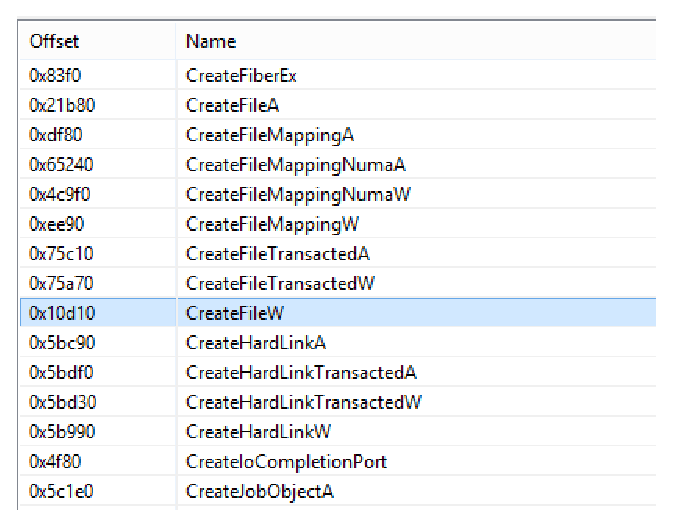
\includegraphics[scale=0.6]{Figures/executable}}
\caption{Information of kernal32.dll}
\label{executable}
\end{figure}

\section{Function Descriptor}
There would be lots of function calls in an execution trace. However, most of them are not of interest. We only concern the function call events of a specific communication method. To be able to identify and reconstruct the functions of interest, the function descriptions is required. Hence, I define the function descriptor as a set of function description:

$cdesc = \lbrace fdesc_1, fdesc_2,...,fdesc_p \rbrace$

Each element $fdesc$ can be defined as:

$fdesc = \lbrace name, type, inparamdesc, outparamdesc \rbrace$

where, $name$ is the function name, $type$ is the function type which can be one of the four types: $open$, $close$, $send$ and $receive$. $inparamdesc$ is the input parameter descriptions illustrating how the registers and memory contents map to a list of parameters of interest(you might not care for all parameters) of a given function call while $outparamdesc$ is the output parameter descriptions. 

Table\ref{functionexample} is an example of a function description. In this example, the function name is ReadFile, it is a function for data receiving, so that function type is $receive$. The parameter description includes the concerned parameters, which are Handle, RecvBuffer and MessageLength. The Handle is an input parameter which is a value stored in the register RCX. The RecvBuffer is an address for the input message stored in the register RAX. The MessageLength is a output value stored in register R9. The value of the input parameters can be retrieved from the memory state on the function call instruction line while the value of the output parameters can be retrieved from the memory state on the function return instruction line. If a parameter is an address instead of value, the address should be retrieved first, then the retrieved address should be used to find the buffer content in the memory state. The function description requires the understanding of the calling convention of the operating system. The Microsoft x64 calling convention can be found in Appendix \ref{convention}. More examples of communication method descriptions will be given in Chapter\ref{chapter:newsol}.

\begin{table}[H]
        \centering
        \caption{An example of a function description}
        \label{functionexample}
        \begin{tabular}{|l|l|l|l|l|l|l|l|}
            \hline
             \multirow{2}{*}{{\textbf{Name}}} & \multirow{2}{*}{{\textbf{Type}}} & \multicolumn{3}{c|}{\textbf{Input Parameter Description}} & \multicolumn{3}{c|}{\textbf{Output Parameter Description}} \\
              \cline{3-8} 
             & & \textbf{Name}& \textbf{Register} &  \textbf{Buffer/Value} & \textbf{Name}& \textbf{Register} &  \textbf{Buffer/Value}  \\
             \hline
             \multirow{2}{*}{ReadFile}
             &\multirow{2}{*}{receive} &  \multirow{2}{*}{Handle} & \multirow{2}{*}{RCX} & \multirow{2}{*}{Value} & RecvBuffer & RDX  & Buffer\\
              \cline{6-8} 
             & & & & & MessageLength & R9  & Value\\
            \hline            
        \end{tabular}
    \end{table}

\section{Function Call Event Reconstruction Algorithm}
In last two sections, I formalized the assembly execution trace and defined the function descriptor of a communication method. To be able to identify a communication, the elements consists a communication should be reconstruction from the traces first. To do so, we need to reconstruct the function call events, in which the function calls' parameters contain the information of a communication, such as the channel identifier, the packets send or received, etc. In this section, I define the function call event and present the algorithm to reconstruct the function call events from the assembly execution trace. 

With the function descriptor and the execution trace as input, the function call event reconstruction algorithm identifies function call entry instruction line and reconstruct the input parameters from the memory state of that line. Then it identifies the function call exit line of the corresponding function call and reconstruct the output parameters from the memory state of the function exit line. After iterate the whole execution trace, the algorithm outputs a sequence of function call events of size $m$ which can be defined as:

$etr = (ev_1, ev_2, ..., ev_m)$

A function call event $ev$ in $etr$ is defined as a triplet:

$ev = <funN, inparas, outparas, type>$

where $funN$ is the function name, $inparas$ includes all the input parameters with the parameter name and value while $outparas$ includes all the output parameters, and $type$ is the event type which inherit from the function description and can be one of the four types: $open$, $send$, $receive$ and $close$.

Note: If the parameter is an buffer, the parameter value is the string from the buffer instead of the buffer address.

An example of a sequence of function call events as the output of this algorithm is shown in Listing\ref{eventsexample}.

\begin{lstlisting}[caption= Example of  $etr$, label=eventsexample]
{funN:CreateNamedPipe, type:open,inparams:{Handler:18, FileName:mypipe}, outparams:{}},
{funN:CreateNamedPipe, type:open,  inparams:{Handler:27,  FileName:Apipe}, outparams:{}},
{funN:WriteFile, type:send, inparams:{Handler:27, SendBuf:Message1}, outparams:{MessageLen:9}},
{funN:WriteFile, type:send, inparams:{Handler:27, SendBuf:Message2}, outparams:{MessageLen:9}},
{funN:ReadFile, type:receive, inparams:{Handler:27}, outparams:{RecvBuf:Message3, MessageLen:9}},
{funN:CloseHandle, type:close, inparams:{Handler:27}, outparams:{}},
{funN:CloseHandle, type:close, inparams:{Handler:18}, outparams:{}}
\end{lstlisting}

Algorithm \ref{eventAlg} shows the detail of the function call event reconstruction algorithm. This algorithm is designed to reconstruct the function call events of a communication method. If multiple communication methods are under investigated, this algorithm can be run multiple times to achieve the goal. Since the function descriptions usually contain a  small number of concerned functions compared to the instruction line number in the execution trace, the time complexity of this algorithm is $O(N)$ , $N$ is the instruction line number of the trace.

\begin{algorithm}[H]
\DontPrintSemicolon
\caption{{\bf Function Event Reconstruction Algorithm} \label{eventAlg}}
\KwIn{ $trace, cdes$}
\KwOut{$etr$}
$etr \leftarrow \emptyset$\; 
Emulate the Execute of each instruction line of the trace;\;
\If{The instruction is a call to a function in the $cdes$}{
   Create an new function call event $ev$;\;
   $ev.funN  \leftarrow fdes.name$;\;
   $ev.type  \leftarrow fdes.type$;\;
   Append all the input parameters of interest to $ev.paras$;\;
   Continue the emulation until the function call return line;\;
   Append all the output parameters of interest to $ev.paras$;\;
   $etr.append(ev)$;\;
}
\KwRet $etr$;\;
\end{algorithm} 

\section{Channel Open Mechanisms}\label{mecha}
The channel open mechanism affect the event stream identification and event stream matching strategy. So I discuss them before presenting those algorithms. The channel open mechanism of named pipe and message queue is relatively simple. In windows implementation, only one function call is related to the handle identification of the stream. However, for TCP and UDP the mechanism is complicated.

\subsection{Named Pipe Channel Open Mechanisms} 
For Named Pipe communication method, a named pipe server is responsible for the creation of the pipe, while clients can connect to the pipe after it was created. The creation of a named pipe returns the handle of that pipe. So the identification of the stream only need to identify the pipe creation function call on the server side and the pipe connection function call on the client side. The handle returned by these function calls will be used later when data is being sent or received to a specified pipe. Figure\ref{namedpipeopen} exemplify the channel set up process for a Named Pipe communication in Windows. 

\begin{figure}[H]
\centerline{\includegraphics[scale=0.5]{Figures/namepipechannelopen}}
 \caption{Channel Open Process for a Named Pipe in Windows}
\label{namedpipeopen}
\end{figure}
    
\subsection{Message Queue Channel Open Mechanisms} 
For the Message Queue communication method, the endpoints of the communication can create the queue or use the existing one. However, both endpoints have to open the queue before they access it. The handle returned by the open queue function will be used later when messages are being sent or received to identify the queue. Figure\ref{msmqopen} exemplify the channel set up process for a Message Queue communication in Windows.
\begin{figure}[H]
\centerline{\includegraphics[scale=0.5]{Figures/msmqchannelopen}}
 \caption{Channel Open Process for a Message Queue in Windows}
\label{msmqopen}
\end{figure}

\subsection{UDP and TCP Channel Open Mechanisms} 
For UDP and TCP communication methods, the communication channel is set up by both endpoints of UDP and TCP channels. The function \textit{socket} should be called to create their own socket on both endpoints. After the socket handles are created, the server endpoint binds the socket to its service address and port by calling the function \textit{bind}. Then the server endpoint calls the function  \textit{accept} to accept the client connection. The client will call the function \textit{connect} to connect to the server. When the function \textit{accept} return successfully, a new socket handle will be generated and returned for further data transfer between the server endpoint and  the connected client endpoint. After all these operations are performed successfully, the channel is established and the data transfer can start. During the channel open stage, server endpoint has two socket handles, the first one is used to listen to the connection from the client, while the second one is created for real data transfer. Figure\ref{channelopen2} exemplify the channel open process for TCP and UDP  in Windows.
    
\begin{figure}[H]
\centerline{\includegraphics[scale=0.6]{Figures/tcpudpchannelopen}}
 \caption{Channel Open Model for TCP and UDP in Windows}
\label{channelopen2}    
\end{figure}

\section{Event Stream Extraction Algorithm}
The function call events in the $etr$ may belong to different endpoint. An event stream is a size $k$ sequence of function call events corresponding to an endpoint of a communication which can be defined as:

$s = (ev_1, ev_2, ..., ev_k)$

$s$ contains the channel open function call events, data send function call events, data receive function call events and channel close function call events. According to the channel open mechanisms discussed in Section\ref{mecha}, the identifier of the channel and the handle of the endpoint can be retrieved from the channel open function call events, while the data streams of the endpoint can be received from send function call events and data receive function call events. So that, given the stream $s$, the endpoint $ e =<handle,  d_r, d_s>$ and the $ch$ of a communication $c$ defined in a communication in Chapter\ref{chapter:mod} can be retrieved.

Note: the definition of $ev$ in $s$ is identical to that in $etr$. However, the event numbering of $s$ is different from $etr$. For example, $ev_1$ in $s$ and $ev_1$ in $etr$ might be different events.

The event stream extraction algorithm is designed to extract the streams from the sequence of function call events. In this algorithm, the stream is need to be identified by the channel open function calls first. Then all other events will be added to the stream.

The input of this algorithm is $etr$ from the function event reconstruction algorithm in Algorithm \ref{eventAlg}. Since the events in $etr$ are reconstructed in sequence of the instructions which are order by the time of occurrence, the events are implicitly sorted by time of occurrence. 

The output of this algorithm is a set of stream of size $p$, which can be defined as:

$str = (s_1, s_2, ..., s_p)$

As to the channel open mechanisms, two different algorithms are designed, one is for Name pipe and Message Queue, while the other is for TCP and UDP. 

\subsubsection{Event Stream Extraction Algorithm for Named Pipe and Message Queue}
This algorithm is designed for extraction of the streams for Named Pipe and Message Queue. Since for each endpoint of the communication, only one channel open function call is needed to identify the endpoint, it is simple to identify the stream once channel open function call event that create the endpoint handle is found. 

The same handle may be reused by other endpoint. However, reuse of the handle would not happen before this stream was closed by the channel close function call event. Therefore, before the detection of the channel close function call, if a new channel open function call with the same returned handle is detected, the second channel open will be ignored. This algorithm handle this by having the $tempstream$ set to keep track of the streams that are still open. Once the stream was closed, the handle can be used by another stream. The time complexity of this algorithm is $O(N)$ , $N$ is the number of events in the trace.

\begin{algorithm}[H]
\DontPrintSemicolon
\caption{{\bf Event Stream Exatraction Algorithm for Named Pipe and Message Queue} \label{streamext1}}
\KwIn{$etr$}
\KwOut{$str$} 
$str \leftarrow \emptyset$\; 
$tempstreams \leftarrow \emptyset$   
\For{$ev \in etr$}{
   $h \leftarrow$the handle identifier from $ev.paras$;\;
   \If{$ev.type = open$}{
      \If{$tempstreams[h]$ not exist}{
         $tempstreams[h] \leftarrow$ a new $s$;\;
         $tempstreams[h].append(ev)$;\;
      }     
   }
   \If{$ev.type = send$ Or $ev.type = receive$}{      
      \If{$tempstreams[h]$ exist}{
         $tempstreams[h].append(ev)$;\;
      }
   }
   \If{$ev.type = close$}{
      \If{$tempstreams[h]$ exist}{
         $tempstreams[h].append(ev)$;\;
         $str.append(tempstreams[h])$;\;        
         remove $tempstreams[h]$ from $tempstreams$;\;
      }
   }         
}
\KwRet $str$;\;
\end{algorithm} 

\subsubsection{Event Stream Extraction Algorithm for TCP and UDP}
This algorithm is designed for extraction of the event streams for TCP and UDP. In the channel open stage, a socket handle created by function call of $socket$ in both client and server. In the server side, this created socket is only used for listening to the client's connection. The listening is accomplished by calling the function $accept$. The input of the $accept$ function call is the listening socket handle, and the output of it is a new data transmission socket handle. This two socket handles are considered to be two handles for two streams, the stream identified by the listening handle is called the parent stream and the one identified by the data transmission handle is called the child stream. However the events in the parents stream contain the information needed for event stream matching algorithm later, so the children stream will inherit all the events from their parents. The time complexity of this algorithm is also $O(N)$, $N$ is the number of events in the trace.

\begin{algorithm}[H]
\DontPrintSemicolon
\caption{{\bf Event Stream Exatraction Algorithm for TCP and UDP} \label{streamext2}}
\KwIn{$etr$}
\KwOut{$str$} 
$str \leftarrow \emptyset$\; 
$tempstreams \leftarrow \emptyset$\;
\For{$ev \in etr$}{
   \If{$ev.funN = socket$}{
      $h \leftarrow$ the handle identifier from $ev.paras$;\;
      \If{$tempstreams[h]$ not exist}{
         $tempstreams[h] \leftarrow$ a new $s$;\tcp*[f]{new a stream}\;
         $tempstreams[h].append(ev)$;\;
      }     
   }  
   \If{$ev.funN = bind$ or $ev.funN = connect$}{
      $h \leftarrow$ the handle identifier from $ev.paras$;\;
      \If{$tempstreams[h]$ exist}{
         $tempstreams[h].append(ev)$;\;
      }     
   }   
   \If{$ev.funN = accept$}{
      $h \leftarrow$ the input listening handle in $ev.paras$;\tcp*[f]{handle of parent stream}\; 
      $hc \leftarrow$ the output data transfer handle in $ev.paras$;\tcp*[f]{handle of child stream}\; 
      \If{$tempstreams[h]$ exist}{  
        \If{$tempstreams[hc]$ not exist}{
            $tempstreams[hc] \leftarrow$ a new $s$;\tcp*[f]{a new stream for the child}\; 
        }
         $tempstreams[hc].append(tempstreams[h])$;\tcp*[f]{append parent's events}\;           
         $tempstreams[hc].append(ev)$;\tcp*[f]{append the current event}\;  
      }     
   }     
   \If{$ev.type = send$ Or $ev.type = receive$}{  
      $h \leftarrow$ the handle identifier from $ev.paras$;\;    
      \If{$tempstreams[h]$ exist}{
         $tempstreams[h].append(ev)$;\;
      }
   }
   \If{$ev.type = close$}{
      $h \leftarrow$ the handle identifier from $ev.paras$;\;
      \If{$tempstreams[h]$ exist}{
         $tempstreams[h].append(ev)$;\;
         $str.append(tempstreams[h])$;\;        
         remove $tempstreams[h]$ from $tempstreams$;\;
      }
   }         
}
\KwRet $str$;\;
\end{algorithm} 


\section{Event Stream Matching Algorithm}\label{streammatch}
The function event extraction algorithm and the event stream extraction algorithms all work on a single execution trace. To identify the communications from the dual\_trace, I need to match two event streams out of those extracted streams from each trace of the dual\_trace. The stream matching algorithm in this section is designed for this purpose. The inputs of the stream matching algorithm are two set of streams $str_0$ and $str_1$ which are output by the event stream extraction algorithm. The output of this algorithm is the matching set. Each matched item in this set contains two streams. 

This matching algorithm is not fully reliable. There are two situations which false negative error might emerge. Take Named Pipe for example, the first situation is multiple(more than two) interacting programs shared the same file as their own channel. Even though the channels are distinct for each communication, but the file is the same one. For example, the Named Pipe server is connected by two clients using the same file. In the server trace, there are two streams found. In each client trace, there is one stream found. For the dual\_trace of server and client1, there will be two possible identified communications, one is the real communication for server and client1 while the other is the false negative error actually is for server and client2. The stream in client1's trace will be matched by two streams in the server's trace. The second situation is the same channel is reused by the different endpoints in the same programs. For example, the Named Pipe server and client finished the first communication and then closed the channel. After a while they re-open the same file again for another communication. The matching is based on the identifiers. So that in this case, there will be two matching. Similar situations can also happen in Message Queue, TCP and UDP communication methods. The data stream verification algorithm discussed in Section\ref{verfication} can reduce the false negative errors. 

The stream matching depends on channel open mechanisms which are different from communication method to communication method. For TCP and UDP the matching can be considered as local address and port of server endpoint matching with remote address and port of client endpoint. For Named Pipe, it uses the file name, while for Message Queue, it uses the queue name as the identifier for matching of two streams. 

The following two subsections discuss the two matching algorithms, one is for Named Pipe and Message Queue, while the other is for TCP and UDP. For both of the algorithms, the time complexity of this algorithm is $O(N*M)$, $N$ and $M$ are the number of streams in both traces.

\subsection{Event Stream Matching Algorithm for Named Pipe and Message Queue}
For Named Pipe and Message Queue, the first function call event $ev_1$ in $s$ is the channel open function which is meaningful for endpoint handle identification. The channel identifier parameter can be found in the $ev_1.paras$. The identifier for Named Pipe is the file name of the pipe while for Message Queue is the queue name. This algorithm finds out all the possible communications regardless some of them might be false negative errors. The input $str_0$ and $str_1$ are two set of streams from the two traces of the dual\_trace. The output $ms$ is a set of two matching streams.

\begin{algorithm}[H]
\DontPrintSemicolon
\caption{{\bf Event Stream Matching Algorithm for Named Pipe and Message Queue} \label{matchAlg1}}
\KwIn{$str_0, str_1$}
\KwOut{$ms$}
$ms \leftarrow \emptyset$\; 
\For{$s_0 \in str_0$}{
\tcc{The first event is the open event}
   $id_0 \leftarrow$ get the channel identifier from $str_0[0].paras$;\;
   \For{$s_1 \in str_1$}{
      $id_1 \leftarrow$ get the channel identifier from $str_1[0].paras$;\;
     \If{$id_0 = id_1$}{
            $c.s_0 = s_0$;\;
            $c.s_1 = s_1$;\;
            $ms.append(c)$;\; 
      }
   }
}
\KwRet $ms$;\;
\end{algorithm} 

\subsection{Event Stream Matching Algorithm for TCP and UDP}
For TCP and UDP, multiple function calls collaborate to create the final communication channel. The local address and port of the server endpoint and the remote address and port of the client endpoint are used to identify the channel. This algorithm gets the local address and port of from the events in the stream of the server and remote address and port from the events in the stream of the client. Then it tries to match two streams by comparing the local and remote address and port. 

\begin{algorithm}[H]
\DontPrintSemicolon
\caption{{\bf Event Stream Matching Algorithm for TCP and UDP} \label{matchAlg2}}
\KwIn{$str_0, str_1$}
\KwOut{$cs$}
$cs \leftarrow \emptyset$\; 
\For{$s_0 \in str_0$}{ 
   $socketev_0 \leftarrow$ the $socket$ function call event from $str_0$;\;   
   $bindev_0 \leftarrow$  the $bind$ function call event from $str_0$;\;
   $connectev_0 \leftarrow$  the $connect$ function call event from $str_0$;\;
   \For{$s_1 \in str_1$}{
      $socketev_1 \leftarrow$ the $socket$ function call event from $str_1$;\;
      $bindev_1 \leftarrow$  the $bind$ function call event from $str_1$;\;
      $connectev_1 \leftarrow$  the $connect$ function call event from $str_1$;\;
\tcp*[f]{$socket$ function call event exists for both server and client streams, $bind$ function call event only exist for server streams while $connect$ function call event only exist for client streams}\;   
     \If{$socketev_0 !=null$ AND $socketev_1 != null$}{ 
\tcp*[f]{$s_0$ is a sever stream, $s_1$ is a client stream}\;
       \If{$bindev_0 != null$ AND $connectev_1 != null$}{
           $localServerAddr \leftarrow$ get serverAddr from $bindev_0.paras$;\;
           $remoteServerAddr \leftarrow$ get serverAddr from $connectev_1.paras$;\; 
       }
\tcp*[f]{$s_1$ is a sever stream, $s_0$ is a client stream}\;
       \ElseIf{$bindev_1 != null$ AND $connectev_0 != null$}{
           $localServerAddr \leftarrow$ get serverAddr from $bindev_1.paras$;\;
           $remoteServerAddr \leftarrow$ get serverAddr from $connectev_0.paras$;\; 
       }
       \If{$localServerAddr = remoteServerAddr$}{                  
            $c.s_0 = s_0$;\;
            $c.s_1 = s_1$;\;
            $cs.append(c)$;\;
          }
       }
    }
 }
\KwRet $cs$;\;
\end{algorithm}

\section{Data Stream Verification Algorithm}\label{verfication}
The data stream verification aims to verify if the data streams of the matched event streams align with the communication properties of the communication model in Chapter\ref{chapter:mod}. The data transfer characteristics divided the communications into reliable and unreliable categories. Named Pipe and TCP fall in the reliable category while Message Queue and UDP fall in the unreliable one. The properties of the models consists of content preservation and timing preservation. So that the verification should cover both preservations: 
\begin{itemize}
\item verify the content preservation of the data in the matched streams. 
\item verify the timing preservation of the data in the matched streams. 
\end{itemize}

To verify the timing preservation, the relative time of the events in both streams is needed. Unfortunately, we can only determine the relative time with in a stream but not crossing two streams. So that it's impossible to verify the timing preservations no matter for reliable or unreliable communications. The verification algorithms discussed in this section will only cover the content preservation.  

The inputs of the data stream verification algorithms are two preliminary matched streams $s_0$ and $s_1$. The output is the a boolean indicating if the streams satisfy the content preservation. All communications don't satisfy the content preservation should be excluded.

For each communication method the verification of the corresponding preservation is applied, That is, for Named Pipe and TCP, the reliable communication preservation need to be verified and for Message Queue and UDP, the unreliable communication preservation need to be verified. The following sub sections present the versification  algorithms for these four communication methods. In each sub section, I discuss the data transfer properties and scenarios of the communication method and then present the developed verification algorithm.

\subsection{Data Stream Verification Algorithm for Named Pipe}
A named pipe provides FIFO communication mechanism for inter-process communication. It can be a one-way or a duplex pipe. \cite{khambattinamed}

The basic data transfer characteristics of Named Pipe are:
\begin{itemize}
  \item Bytes are received in order
  \item Bytes sent as a segment can be received in multiple segments(the opposite is not true)
  \item No data duplication
  \item If a sent segment is loss, all the following segments will lost(this happen when the receiver disconnect from the channel) 
  
\end{itemize}

Based on these characteristics, the data transfer scenarios of Named pipe can be exemplified in Figure\ref{namedpipe}. 
\begin{figure}[H]
\centerline{\includegraphics[scale=0.4]{Figures/namedpipe}}
\caption{Data Transfer Scenarios for Named Pipe}
\label{namedpipe}
\end{figure}

The content preservation verification is trivial as comparing the concatenation of the packet content of the sent events in a stream to the the concatenation of the packet content of the receive events in the other stream, which is presented in Algorithm \ref{channelopen2}. Since the concatenation need to go through the events in the streams, the time complexity of this algorithm is also $O(N)$, $N$ is the total number of data transfer events in the two streams.

\begin{algorithm}[H]
\DontPrintSemicolon
\caption{{\bf Data Stream Verification of Named Pipe} \label{dataAlg1}}
\KwIn{$s_0, s_1$}
\KwRet{$satisfied$}\;
$send_0 \leftarrow$ concatenation of the payload of send function call events in $s_0$;\;
$send_1 \leftarrow$ concatenation of the payload of send function call events in $s_1$;\;
$receive_0 \leftarrow$ concatenation of the payload of receive function call events in $s_0$;\;
$receive_1 \leftarrow$ concatenation of the payload of receive function call events in $s_1$;\;
\If{$receive_1$ is prefix of $send_0$ AND $receive_0$ is prefix of $send_1$ }{
   \KwRet True;\;
}
\Else{
    \KwRet False;\;
}
\end{algorithm} 

\subsection{Data Stream Verification Algorithm for TCP}
TCP is the most fundamental reliable transport method in computer networking. TCP provides reliable, ordered, and error-checked delivery of a stream of octets between applications running on hosts in an IP network. The TCP header contains the sequence number of the sending octets and the acknowledge sequence this endpoint is expecting from the other endpoint(if ACK is set). The re-transmission mechanism is based on the ACK. 

The basic data transfer characteristics of TCP are:
\begin{itemize}
  \item Bytes received in order
  \item No data lost(lost data will be re-transmitted)
  \item No data duplication
  \item Bytes sent in packet and received in packet, no re-segmentation
\end{itemize}

Based on these characteristics,  the data transfer scenarios of TCP can be exemplified in Figure\ref{tcp}.
\begin{figure}[H]
\centerline{\includegraphics[scale=0.4]{Figures/tcp}}
 \caption{Data Transfer Scenarios for TCP}
\label{tcp}
\end{figure}

Regrading to the data transfer properties of TCP, the verification can be restricted to packet to packet. If all the send and receive events of the two streams can be matched, we can assert that the content preservation are satisfied. The verification algorithm of TCP is presented in Algorithm \ref{dataAlg2}. The time complexity of this algorithm is also $O(N)$, $N$ is the number of data transfer events in a stream.

\begin{algorithm}[H]
\DontPrintSemicolon
\caption{{\bf Data Stream Verification of TCP} \label{dataAlg2}}
\KwIn{$s_0, s_1$}
\KwRet{$satisfied$}\;
$sends_0 \leftarrow$ all sent events of $s_0$ in sequence;\;
$sends_1 \leftarrow$ all sent events of $s_1$ in sequence;\;
$receives_0 \leftarrow$ all receive events of $s_0$ in sequence;\;
$receives_1 \leftarrow$ all receive events of $s_1$ in sequence;\;
\If{$sends_0.size != receives_1.size$ Or $sends_1.size != receives_0.size$ }{
   \KwRet False;\;
}
\For{$i \in {0..sends_0.size}$}{
     \If{$sends_0[i].payload != receives_1[i].payload$}{
       \KwRet False;\;
   }
}
\For{$i \in {0..sends_1.size}$}{
     \If{$sends_1[i].payload != receives_0[i].payload$}{
       \KwRet False;\;
   }
}
 \KwRet True;\;
\end{algorithm} 



\subsection{Data Stream Verification Algorithm for Message Queue}
Message Queuing is a communication method to allow applications which are running at different times across heterogeneous networks and systems that may be temporarily offline can still communicate with each other. Messages are sent to and read from queues by applications. Multiple sending applications can send messages to and multiple receiving applications can read messages from one queue.\cite{redkar2004pro} In this work, only one sending application versus one receiving application case is considered. Multiple senders to multiple receivers scenario can be divided into multiple sender and receiver situation. Both applications of a communication can send to and receive from the channel.

The basic data transfer characteristics of Message Queue are:
\begin{itemize}
  \item Bytes sent in packet and received in packet, no bytes re-segmented
  \item Packets can lost
  \item Packets received in order
  \item No data duplication
\end{itemize}
Based on these characteristics, the data transfer scenarios of Message Queue can be exemplified in Figure\ref{msmq}.
\begin{figure}[H]
\centerline{\includegraphics[scale=0.4]{Figures/msmq}}
\caption{Data Transfer Scenarios for Message Queue}
\label{msmq}
\end{figure}

To verify the content preservation of the unreliable communication, Algorithm \ref{dataAlg3} tries to find the match sent packet in the other stream for each received packet. If any of the received packet can not be match, the content preservation is not satisfied. Since the sent packets are received in order, the searching for each received packet will start from the next index of the last matching sent packet. 

\begin{algorithm}[H]
\DontPrintSemicolon
\caption{{\bf Data Stream Verification of Message Queue } \label{dataAlg3}}
\KwIn{$s_0, s_1$}
\KwRet{$satisfied$}\;
$sends_0 \leftarrow$ all sent events of $s_0$ in sequence;\;
$sends_1 \leftarrow$ all sent events of $s_1$ in sequence;\;
$receives_0 \leftarrow$ all receive events of $s_0$ in sequence;\;
$receives_1 \leftarrow$ all receive events of $s_1$ in sequence;\;
\If{$sends_0.size < receives_1.size$ Or $sends_1.size < receives_0.size$ }{
   \KwRet False;\;
}
$lastMatchIndex = 0$;\;
\For{$i \in {0..receives_1.size}$}{
     $tempIndex = lastMatchIndex$;\;
     \For{$j \in {lastMatchIndex+1..sends_0.size}$}{
             \If{$sends_0[j].payload = receives_1[i].payload$}{
                      $lastMatchIndex = j$;\;
                      break the inner For loop;\;
            }  
     }   
\tcp*[f]{This received packet can not be matched by any sent packet}\;      
     \If{$tempIndex = lastMatchIndex$}{
                      \KwRet False;\;
            }     
}     
$lastMatchIndex = 0$;\;
\For{$i \in {0..receives_0.size}$}{
     $tempIndex = lastMatchIndex$;\;
     \For{$j \in {lastMatchIndex+1..sends_1.size}$}{
             \If{$sends_1[j].payload = receives_0[i].payload$}{
                      $lastMatchIndex = j$;\;
                      break the inner For loop;\;
            }  
     }   
     \If{$tempIndex = lastMatchIndex$}{
                      \KwRet False;\;
            }     
}  
 \KwRet True;\;
\end{algorithm} 

The time complexity of this algorithm is $O(N^2+M^2)$, $N$ and $M$ are the numbers of data sent events of the two streams.

\subsection{Data Stream Verification Algorithm for UDP}
UDP is a widely used unreliable transmission method in computer networking. It is a simple protocol mechanism, which has no guarantee of delivery, ordering, or duplicate protection. This transmission method is suitable for many real time systems. 

The basic data transfer characteristics of UDP are:
\begin{itemize}
  \item Bytes sent in packet and received in packet, no re-segmentation
  \item Packets can lost
  \item Packets can be duplicated
  \item Packets can arrive receiver out of order
\end{itemize}

Based on these characteristics, the data transfer scenarios of UDP can be exemplified in Figure\ref{upd}.
\begin{figure}[H]
\centerline{\includegraphics[scale=0.4]{Figures/udp}}
 \caption{Data Transfer Scenarios for UDP}
\label{upd}
\end{figure}

Similar to Message Queue, Algorithm \ref{dataAlg4} try to find the match sent packet in the other stream for each received packet. If any of the received packet can not be match, the content preservation is not satisfied. However, due to the disordering can happen in UDP, the searching for each received packet will not constraint the searching index. But the matched sent packet will excluded from the following searching, which means each sent packet can only match to one received packet.

\begin{algorithm}[H]
\DontPrintSemicolon
\caption{{\bf Transmitted Verification of UDP} \label{dataAlg4}}
\KwIn{$s_0, s_1$}
\KwRet{$satisfied$}\;
$sends_0 \leftarrow$ all sent events of $s_0$ in sequence;\;
$sends_1 \leftarrow$ all sent events of $s_1$ in sequence;\;
$receives_0 \leftarrow$ all receive events of $s_0$ in sequence;\;
$receives_1 \leftarrow$ all receive events of $s_1$ in sequence;\;
\If{$sends_0.size < receives_1.size$ Or $sends_1.size < receives_0.size$ }{
   \KwRet False;\;
}
\For{$i \in {0..receives_1.size}$}{
    $matchFlag = False$;\;
     \For{$j \in {0..sends_0.size}$}{
             \If{$sends_0[j].payload = receives_1[i].payload$}{
                      $matchFlag = True$;\;
                      delete the packet from $sends_0$
                      break the inner For loop;\;
            }  
     }   
\tcp*[f]{This received packet can not be matched by any sent packet}\;      
     \If{$matchFlag = False$}{
                      \KwRet False;\;
            }     
}     
\For{$i \in {0..receives_0.size}$}{
    $matchFlag = False$;\;
     \For{$j \in {0..sends_1.size}$}{
             \If{$sends_1[j].payload = receives_0[i].payload$}{
                      $matchFlag = True$;\;
                      delete the packet from $sends_0$
                      break the inner For loop;\;
            }  
     }   
     \If{$matchFlag = False$}{
                      \KwRet False;\;
            }     
} 
 \KwRet True;\;
\end{algorithm} 

The time complexity of this algorithm is $O(N^2+M^2)$, $N$ and $M$ are the numbers of data sent transfer events in the two streams.

\section{Communication Identification Process}
The general communication identification of the dual\_trace consist of the algorithms presented previously in this chapter and can be summarized as the follow steps with the corresponding algorithm for each communication categories(i.e. reliable or unreliable) and each communication methods:

\textbf{Step 1.} Execute the Function Event Reconstruction algorithm to the two traces in the dual\_trace

\textbf{Step 2.} Execute the Stream Exaction Algorithm to the both traces 

\textbf{Step 3.} Use the Stream Matching Algorithm to match the streams of the two traces

\textbf{Step 4.} Verify the matched streams by the their satisfaction of the content preservation

\textbf{Step 5.}  Include the matched streams that satisfy the preservation

\textbf{Step 6.}  Retrieve the endpoint $e =<handle,  d_r, d_s>$ and channel identifier $ch$ from the matched streams and output a set the communications. (No corresponding algorithm for this step since the retrieval is only reorganize the information in the streams and is trivial)


\section{Limitation of the Identification}
The Identification discussed in this chapter is not perfect. It has two major limitations:
\begin{itemize}
    \item The timing preservation of the communication is not verified.
    \item Due to the data transmitted in two communications can be identical(or their difference can not be tell by the content verification), the false negative error of the identification can not be eliminated. Figure\ref{secondlevelmatching} indicates the ineffective and effective identification scenarios. 
\end{itemize}



\begin{figure}[H]
\centerline{\includegraphics[scale=0.5]{Figures/secondlevelmatching}}
 \caption{Communication Identification Scenarios}
\label{secondlevelmatching}
\end{figure}




	\externaldocument{../3/chapter_modeling}
\externaldocument{../4/chapter_algorithm}
\startchapter{Feature Prototype On Atlantis}
\label{chapter:newsol}
In this chapter, I present the design of the feature prototype of communication identification from the dual\_trace. This prototype implemented some of the algorithms described in Chapter\ref{chapter:alo} as well as the user interfaces.

This feature prototype is implemented on Atlantis to utilize its other features, such as ``memory reconstruction", ``function inspect" and ``views synchronization". Figure \ref{executable} shows the decoded information needed to identify a function call of interest from the trace. The feature ``function inspect" of Atlantis provide this decoding functionality. In the function call event reconstruction algorithm, the parameters of a function call is are retrieved from the memory state. The ``memory reconstruction" functionality of Atlantis which compute the memory state of the instruction line efficiently makes this retrieval easier. Moreover, the ``views synchronization" ability of Atlantis benefit the user when they are navigating and viewing the communication identification result.

This prototype consists of four components: 1) user setting for the function descriptors of the communication methods. 2) a view that can parallel display both traces in the dual\_trace. 3) two features: stream extraction and communication identification. 4) stream extraction or communication identification result navigation.

To analyse a dual\_trace, the user need to 1) open two traces in the parallel editor(developed in this prototype), 2) import the dynamic linked library file for each trace(existing feature of Atlantis), 3) perform the stream extraction or communication identification operations(developed in this prototype), and finally 4) inspect the operation results(by the operation menu developed in this prototype and the navigation functions existing in Atlantis).

Before describing the detail of each of these component, I provide two use cases corresponding to the two main features: stream extraction and communication identification of this prototype as shown in Table \ref{usecase1} and Table \ref{usecase2}.

\begin{table}[H]
  \centering
  \caption{Use Case 1: Extract Streams from the Dual\_trace}
  \label{usecase1}
  \begin{tabular}{|l|p{13cm}|}
      \hline
       \textbf{Name} & Analysis streams of a communication method from the Dual\_trace\\
       \hline
       \textbf{Description} & A user captured two assembly execution traces of two interacting program and need to analysis them by extracting all communication streams of each of the traces and inspecting the extraction results \\
       \hline
              \textbf{Actor} & A Software Security Engineer \\
       \hline
       \textbf{Precondition} & The user has two assembly execution trace and the .dll files on the systems where the programs of the captured traces were running\\
       \hline
       \textbf{Main Course}& 1. The user input the function descriptor for the communication methods of interest to the Json format setting file\\
        & 2. The user open one of the trace in Atlantis\\
       &  3. The user open the other trace as the dual\_trace of the first one\\
       & 4. The two opened traces are presented in the parallel editor view\\
       & 5. The user load the related .dll files which contains the information of the functions in the function descriptors for both opened trace\\
       & 6. The user select the operation ``Stream Extraction" in the ``Dual\_Trace Tool" menu.\\
       & 7. Atlantis prompt a dialogue window giving the user all the communication methods in the function descriptor setting file as option\\
       & 8. The user select the communication methods which they want to analyse and click the ``OK" bottom\\
       & 9. Atlantis extract the streams for both traces and list the result in ``Communication view"\\
       & 10. The user expand the result in the ``Communication view"\\
       & 11. The user select one function call event in a stream and double click the entry\\
       & 12. Atlantis navigation to the corresponding instruction line in the trace and synchronize all other views\\
      \hline               
  \end{tabular}
\end{table}

\begin{table}[H]
  \centering
  \caption{Use Case 2: Identify Communications from the Dual\_trace}
  \label{usecase2}
  \begin{tabular}{|l|p{13cm}|}
      \hline
       \textbf{Name} & Analysis communications of a communication method from the Dual\_trace\\
       \hline
       \textbf{Description} & A user captured two assembly execution traces of two interacting program and need to analysis them by identify all communications of the dual\_trace and inspecting the extraction results \\
       \hline
              \textbf{Actor} & A Software Security Engineer \\
       \hline
       \textbf{Precondition} & The user has two assembly execution trace and the .dll files on the systems where the programs of the captured traces were running\\
       \hline
       \textbf{Main Course}& 1. The user input the function descriptor for the communication methods of interest to the Json format setting file\\
        & 2. The user open one of the trace in Atlantis\\
        &  3. The user open the other trace as the dual\_trace of the first one\\
       & 4. The two opened traces are presented in the parallel editor view\\
       & 5. The user load the related .dll files which contains the information of the functions in the function descriptors for both opened trace\\
       & 6. The user select the operation ``Communication Identification" in the ``Dual\_Trace Tool" menu\\
       & 7. Atlantis prompt a dialogue window giving the user all the communication methods in the function descriptor setting file as option\\
       & 8. The user select the communication methods which they want to analyse and click the ``OK" bottom\\
       & 9. Atlantis identify the communication for both traces and list the result in ``Communication view"\\
       & 10. The user expand the result in the ``Communication view"\\
       & 11. The user select one function call event in a stream and double click the entry\\
       & 12. Atlantis navigation to the corresponding instruction line in the trace and synchronize all other views\\
      \hline               
  \end{tabular}
\end{table}

\section{User Setting of the Function Descriptors}\label{functionset}
In Section \ref{cdesc}, I defined a function descriptor as a set of function descriptions for a communication method. The communication identification approach can identify the communications described by the function descriptor from the dual\_trace.

However, the communication method description for a communication method can be different depends on the implementation solution of the communication method. Furthermore, there are so many communication methods in the real world, it is impossible to pre-define all of them for the users. Instead, a configuration file in Json format is provided for the users to define their communication methods of interest and the corresponding function descriptors. A default template is given for user reference, this default template is generated by Atlantis when it was launched and stored in the .tmp folder in the trace analysis project folder. The users can modify this template as to the communication methods of interest. The default template example can be find in Section\ref{funcset}.

The function descriptors in this setting file will be the input for the stream extraction and communication identification features. When the user use this two features, the list of the communication methods provided in the setting files will be presented to them. They can select one or more communication methods to be analysed. 

In the following subsections, function descriptor examples are presented as user reference to how to design their own function descriptor for a communication method.

\subsection{Communication Methods' Implementation in Windows}\label{windows}
Learning the implementation of a communication is necessary to obtain the function descriptor of the communication method.  In this section, I present the result of investigation about the implementation of the four communication methods: Named Pipe, Message Queue, TCP and UDP in Windows. In the investigation, I reviewed the Windows APIs of the communication methods and their example code. By doing so, I obtained the function descriptors of these methods can be designed by this investigation.

Windows API set is very sophisticated. Moreover, multiple solutions are provided to fulfil a communication method. It is impossible to enumerate all solutions for each communication method. I only investigated the most basic usage provided in Windows documentation. For each communication method, a function descriptor with a list of system function descriptions is provided for reference. The functions in the descriptors are supported in most Windows operating systems, such as Windows 8, Window 7. The provided function descriptor of a communication method should only be considered as an example for that communication method. With the understanding of this, it should be fairly easy to obtain the function descriptors for other solutions of that communication method or other communication methods. 

Note that, the instances of the descriptors only demonstrate Windows C++ APIs. But the idea of the function descriptor is generalizable to other operating systems with the effort of understanding the APIs of those operating systems.

\subsubsection{Windows Calling Convention}
The Windows calling convention is important to know in this research. The communication identification from dual\_trace in assembly level relies not only on the system function names but also the key parameter values. In the assembly level execution traces, the parameter values is captured in the memory changes and register changes of the instructions but without any information indicating which registers or memory addresses are holding this parameters. The calling convention tells us where the parameters are stored. So that we can find them in the memory state while emulate the execution of the trace. Calling Convention is various for operating systems and the programming language. I used dual-trace of Microsoft* x64 programs for case study in this research. The Microsoft* x64 example calling convention is listed in Appendix \ref{convention}.

\subsubsection{Named Pipes}
In Windows, a named pipe is a communication method for the pipe server and one or more pipe clients. The pipe has a name, can be one-way or duplex. Both the server and clients can read or write into the pipe.\cite{WinNamedpipe} In this work, I only consider one server versus one client communication. One server to multiple clients scenario can always be divided into multiple server and client communications thanks to the characteristic that each client and server communication has a separate conduit. The server and client are endpoints in the communication. We call the server ``server endpoint" while the client ``client endpoint".  The server endpoint and client endpoint of a named pipe share the same pipe name, but each endpoint has its own buffers and handles. 

There are two modes for data transfer in the named pipe communication method, synchronous and asynchronous.  Modes affect the functions used to complete the send and receive operation. Both descriptors for both synchronous mode and asynchronous mode are provided. The create channel functions for both modes are the same but with different input parameter value. The functions for send and receive message are also the same for both cases. However, the operation of the send and receive functions are different for different modes. In addition, an extra function \textit{GetOverlappedResult} is being called to check if the sending or receiving operation finish, the output message will be stored in the overlap structure whose memory address saved in the function's output parameter Overlap Structure Address. Table\ref{namesyn} is the function descriptor for synchronous mode while Table\ref{nameasyn} is the function descriptor asynchronous mode of Named pipe.

\begin{table}[H]
  \centering
  \caption{Function Descriptor for Synchronous Named Pipe}
  \label{namesyn}
  \begin{tabular}{|l|l|l|l|l|l|l|l|}
\hline
             \multirow{2}{*}{{\textbf{Name}}} & \multirow{2}{*}{{\textbf{Type}}} & \multicolumn{3}{c|}{\textbf{Input Parameter Description}} & \multicolumn{3}{c|}{\textbf{Output Parameter Description}} \\
              \cline{3-8} 
             & & \textbf{Name}& \textbf{Register} & \textbf{Addr/Val} & \textbf{Name}& \textbf{Register} &  \textbf{Addr/Val}  \\
             \hline
      CreateNamedPipe
       &open & FileName & RCX  & Addr &  Handle & RAX & Val\\
      \hline         
      CreateFile
       &open & FileName & RCX & Addr&  Handle & RAX & Val\\ 
      \hline              
      \multirow{2}{*}{WriteFile}
       &\multirow{2}{*}{send} &  Handle & RCX & Val & \multirow{2}{*}{Length} & \multirow{2}{*}{R9} & \multirow{2}{*}{Val}\\
        \cline{3-5} 
       & & SendBuf & RDX & Addr & & &\\
      \hline            
      \multirow{2}{*}{ReadFile}
       &\multirow{2}{*}{receive} &  Handle & RCX & Val& \multirow{2}{*}{Length} & \multirow{2}{*}{R9} & \multirow{2}{*}{Val}\\
        \cline{3-5} 
       & & RecvBuf & RDX  & Addr & & &\\
      \hline            
      CloseHandle &
       close &  Handle & RCX & Val & & &\\
      \hline            
      DisconnectNamedPipe &
      close &  Handle & RCX & Val & & &\\
      \hline               
  \end{tabular}
\end{table}

\begin{table}[H]
  \centering
  \caption{Function Descriptor for Asynchronous Named Pipe}
  \label{nameasyn}
\begin{tabular}{|l|l|l|l|l|l|l|l|}
\hline
             \multirow{2}{*}{{\textbf{Name}}} & \multirow{2}{*}{{\textbf{Type}}} & \multicolumn{3}{c|}{\textbf{Input Parameter Description}} & \multicolumn{3}{c|}{\textbf{Output Parameter Description}} \\
              \cline{3-8} 
             & & \textbf{Name}& \textbf{Register} & \textbf{Addr/Val} & \textbf{Name}& \textbf{Register} &  \textbf{Addr/Val}  \\
             \hline
      CreateNamedPipe
       &open & FileName & RCX  & Addr &  Handle & RAX & Val\\
      \hline         
      CreateFile
       &open & FileName & RCX & Addr&  Handle & RAX & Val\\ 
      \hline              
      \multirow{2}{*}{WriteFile}
       &\multirow{2}{*}{send} &  Handle & RCX & Val & \multirow{2}{*}{Length} & \multirow{2}{*}{R9} & \multirow{2}{*}{Val}\\
        \cline{3-5} 
       & & SendBuf & RDX & Addr & & &\\
      \hline            
      \multirow{2}{*}{ReadFile}
       &\multirow{2}{*}{receive} &  Handle & RCX & Val& \multirow{2}{*}{Length} & \multirow{2}{*}{R9} & \multirow{2}{*}{Val}\\
        \cline{3-5} 
       & & RecvBuf & RDX  & Addr & & &\\
      \hline    
           GetOverlappedResult &
       receive &  Handle & RCX & Val &OverlapStruct &RDX & Addr\\
      \hline     
      CloseHandle &
       close &  Handle & RCX & Val & & &\\
      \hline            
      DisconnectNamedPipe &
      close &  Handle & RCX & Val & & &\\
      \hline               
  \end{tabular}  
\end{table}

\subsubsection{Message Queue}
Similar to Named Pipe, Message Queue's implementation in Windows also has two modes, synchronous and asynchronous. Moreover, the asynchronous mode further divides into two operations, one with callback function while the other without. With the callback function, the callback function would be called when the send or receive operations finish. Without callback function, the general function \textit{MQGetOverlappedResult} should be called by the endpoints to check if the message sending or receiving operation finish, the parameter in RCX of this function call is a structure consist of the handle as an input parameter and the overlap structure as an output parameter. Table\ref{msmqsynfunctions} is the function descriptor for synchronous mode while Table\ref{msmqasynfunctions} is the function descriptor for the asynchronous mode without callback. With callback function situation is not elaborated here.

\begin{table}[H]
  \centering
  \caption{Function Descriptor for Synchronous Message Queue}
  \label{msmqsynfunctions}
\begin{tabular}{|l|l|l|l|l|l|l|l|}
\hline
             \multirow{2}{*}{{\textbf{Name}}} & \multirow{2}{*}{{\textbf{Type}}} & \multicolumn{3}{c|}{\textbf{Input Parameter Description}} & \multicolumn{3}{c|}{\textbf{Output Parameter Description}} \\
              \cline{3-8} 
             & & \textbf{Name}& \textbf{Register} & \textbf{Addr/Val} & \textbf{Name}& \textbf{Register} &  \textbf{Addr/Val}  \\
             \hline
      MQOpenQueue
       &open & QueueName & RCX  & Addr &  Handle & RAX & Val\\
      \hline                     
      \multirow{2}{*}{MQSendMessage}
       &\multirow{2}{*}{send} &  Handle & RCX & Val &  &  & \\
       \cline{3-5}
      & & MessStruct& RDX&Addr &  &  & \\
      \hline            
      MQReceiveMessage
       &receive&  Handle & RCX & Val& MessStruct& RDX&Addr\\
      \hline       
      MQCloseQueue &
       close &  Handle & RCX & Val & & &\\
      \hline                          
  \end{tabular}   
\end{table}

\begin{table}[H]
  \centering
  \caption{Function Descriptor for Asynchronous Message Queue}
  \label{msmqasynfunctions}
\begin{tabular}{|l|l|l|l|l|l|l|l|}
\hline
             \multirow{2}{*}{{\textbf{Name}}} & \multirow{2}{*}{{\textbf{Type}}} & \multicolumn{3}{c|}{\textbf{Input Parameter Description}} & \multicolumn{3}{c|}{\textbf{Output Parameter Description}} \\
              \cline{3-8} 
             & & \textbf{Name}& \textbf{Register} & \textbf{Addr/Val} & \textbf{Name}& \textbf{Register} &  \textbf{Addr/Val}  \\
             \hline
      MQOpenQueue
       &open & QueueName & RCX  & Addr &  Handle & RAX & Val\\
      \hline                     
      \multirow{2}{*}{MQSendMessage}
       &\multirow{2}{*}{send} &  Handle & RCX & Val &  &  & \\
       \cline{3-5}
      & & MessStruct& RDX&Addr &  &  & \\
      \hline            
      MQReceiveMessage
       &receive&  Handle & RCX & Val& MessStruct& RDX&Addr\\
      \hline    
      MQGetOverlapResult &
       receive &  Handle & RCX & Addr & Overlapstr& RCX&Addr\\
      \hline      
      MQCloseQueue &
       close &  Handle & RCX & Val & & &\\
      \hline                          
  \end{tabular}   
\end{table}


    
\subsubsection{TCP and UDP}
In Windows programming, these two methods shared the same set of APIs regardless the input parameter values and operation behaviour are different. In Windows socket solution, one of the two endpoints is the server while the other one is the client. Table \ref{tcpupdfunctions} is the function descriptor for UDP or TCP communication. 

\begin{table}[H]
  \centering
  \caption{Function Descriptor for for TCP and UDP}
  \label{tcpupdfunctions}
\begin{tabular}{|l|l|l|l|l|l|l|l|}
\hline
             \multirow{2}{*}{{\textbf{Name}}} & \multirow{2}{*}{{\textbf{Type}}} & \multicolumn{3}{c|}{\textbf{Input Parameter Description}} & \multicolumn{3}{c|}{\textbf{Output Parameter Description}} \\
              \cline{3-8} 
             & & \textbf{Name}& \textbf{Register} & \textbf{Addr/Val} & \textbf{Name}& \textbf{Register} &  \textbf{Addr/Val}  \\
             \hline
      socket
       &open &  &   &  &  Socket & RAX & Val\\
      \hline
      bind
       &open & Socket &  RCX & Val &  ServerAddrAndPort & RDX & Addr\\
      \hline   
            connect
       &open & Socket &  RCX & Val &  ServerAddrAndPort & RDX & Addr\\
      \hline   
     accept
       &open &  ListenSocket & RCX & Val & ConnectSocket & RAX & Val\\
      \hline                    
      \multirow{2}{*}{send}
       &\multirow{2}{*}{send} &  Handle & RCX & Val &  &  & \\
       \cline{3-5}
      & & SendBuf& RDX&Addr &  &  & \\
      \hline            
      recv
       &receive&  Handle & RCX & Val& RecvBuf& RDX&Addr\\
      \hline      
      closesocket &
       close &  Handle & RCX & Val & & &\\
      \hline                          
  \end{tabular}    
\end{table}

\section{Parallel Editor View For Dual\_Trace}
The dual\_trace consist of two execution traces which are interacting with each other. Presenting them in the same view makes the analysis for the user much easier. To open parallel editor view, the user need to open one trace as the normal one and the other as the dual\_trace of the opened one. A new menu option in the project navigation view are added to open the second trace as the dual\_trace of the active trace. The implementation of the parallel editor take the advantage of the existing SWT of Eclipse plug-in development. The detail of the implementation can be found in Appendix \ref{paralleleditor}. Figure \ref{opendualtracemenu} shows this menu option and Figure \ref{paralleleditor} shows the parallel editor view.

\begin{figure}[H]
\centerline{\includegraphics[scale=0.4]{Figures/opendualtracemenu}}
 \caption{Menu Item for opening Dual\_trace}
\label{opendualtracemenu}
\end{figure}

\begin{figure}[H]
\centerline{\includegraphics[scale=0.6]{Figures/paralleleditor}}
 \caption{Parallel Editor View}
\label{paralleleditor}
\end{figure}

\section{Features}
I implemented two features. The first one is stream extraction corresponding to the stream extraction algorithm presented in Chapter\ref{chapter:alo} for both traces in the dual\_trace. The other one is the communication identification corresponding to the overall communication process discussed in Chapter\ref{chapter:alo}. The implementation of these two features relies on the existing ``function inspect" feature of Atlantis. The called functions' name can be inspected  by  search of the symbolic name in the executable binary or any DLLs which used by the program at the time when it is traced. By importing the DLLs and executable binary, Atlantis can recognize the function call from the execution trace by the function names. Therefore the corresponding Dlls or executable binaries for both traces in the dual\_trace have to be loaded into Atlantis before conducting the identification.

A new menu ``Dual\_trace Tool" with three menu options is designed for these two features. In this menu, ``Stream Extraction" is for the operation of stream extraction and ``Communication Identification" is for the operation of communication identification. For both of these two operation ``Load Library Exports" has to be run before for both traces. Currently, the ``Load library export"  operation can only load libraries for the trace in the active editor. So ``Load library export"  in the menu has to be run twice separately for each trace of the dual\_trace.  Figure\ref{dualtracetoolmenu} shows this new menu in Atlantis. When the user perform ``Stream Extraction" or ``Communication Identification", there will be a prompt dialog as shown in Figure \ref{methods} which asks the user what communication methods they want to analyse from the dual\_trace. This list is provided by the configuration file I mention in Section \ref{functionset}. The user can select one or multiple methods. 

\begin{figure}[H]
\centerline{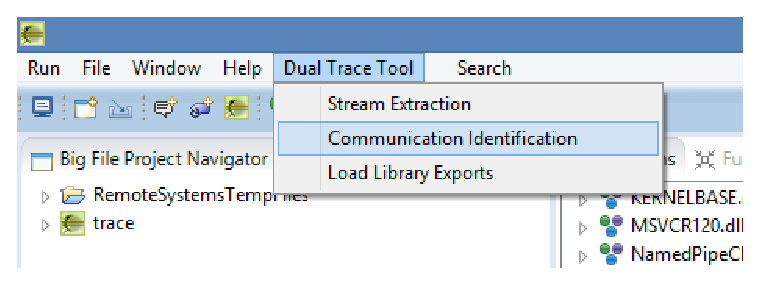
\includegraphics{Figures/dualtracetoolmenu}}
 \caption{Dual\_trace Tool Menu}
\label{dualtracetoolmenu}
\end{figure}

\begin{figure}[H]
\centerline{\includegraphics[scale=0.8]{Figures/methods}}
 \caption{Prompt Dialog for Communication Selection}
\label{methods}
\end{figure}

A new view named ``Communication" is designed for presenting the result of the extracted streams and the identified communications. Since the user can have multiple selection for communication methods of interest, the output identification result contains all the identified communications or streams of all selected communication methods and the results are clustered by methods. There are two sub tables in this view, the left one is for presenting the extracted the streams result while the left one is for presenting communication identification result. The reason for putting this two result in the same view is for easy access and comparison of the data for the users. Figure \ref{idenview} shows this view with result data in it. Each time when the user rerun the features the result in the corresponding table will be refreshed to show only the latest identification result. But the other table will not be affected. For example, if the user run the ``Stream Extraction" feature first, the stream result will show on the left table of the view. And then the user run the ``communication Identification", the communication identification result will be shown on the right table while the left one still holding the last stream result.

\begin{figure}[H]
\centerline{\includegraphics[scale=0.7]{Figures/idenview}}
 \caption{Communication View for Result}
\label{idenview}
\end{figure}

\section{Result Navigation}
Atlantis is a analysis environment that has various views to allow user access to different information from the trace, such as the memory and register state of the current instruction line. Moreover, these views synchronize automatically with the editor view. These functionality and information also benefit the communication analysis of the dual\_trace. Providing the user a way to navigate from the result to the traces in the editors allows them to take advantage of the current existing functionality of Atlantis and make their analysis of the dual\_trace more efficient.

In the result list, each event entry is corresponding to a function call. The functions were called at function call line and all the inputs of the function calls can be recovered from the memory state of this instruction line. The functions returned at the return instruction lines, all the outputs of the function calls can be recovered in the memory state of the the return instruction line. From the event entries, this implementation provide two different ways for the user to navigate back to where the function begins and ends. When the user ``double click" on an entry, it will bring the user to the start line of the function in the corresponding trace editor. When the the right click on the event entry, a prompted menu with the option ``Go To Line of Function End" will show up as in Figure \ref{gotoend}. Clicking on this option will bring the user to the return line of this function in the trace editor. All other views update immediately with this navigation. 

\begin{figure}[H]
\centerline{\includegraphics{Figures/gotoend}}
 \caption{Right Click Menu on Event Entry}
\label{gotoend}
\end{figure}

Moreover, the ``remove" option as shown in Figure \ref{remove} in the right click menu on the ``stream“ or ``communication" entries is provided for the user to remove the selected ``stream" or ``communication" entry. This provides the user the flexibility to get rid of the data that they don't care.

\begin{figure}[H]
\centerline{\includegraphics[scale=0.7]{Figures/remove}}
 \caption{Right Click Menu on Event Entry}
\label{remove}
\end{figure}


	\externaldocument{../appendix/chapter_app}
\externaldocument{../4/chapter_algorithm}
\startchapter{Evaluation}
\label{chapter:Exp}
This evaluation aimed to experimentally evaluate the model for communication analysis and the identification algorithms. The evaluation only focus on evaluating the correctness and efficiency of the model and algorithm. User case study is not included in this thesis and can be the future work. The feature prototype implementation is not evaluated and can be part of the user case study. In this section, I describe the design of the evaluation.  Then the results of the experiment evaluation are provided and concluded.

\subsection{Experiment Evaluation Design}
Two experiments are conducted for this evaluation.  All the programs in these two experiments were written in C++ and the source code can be found in Section\ref{expcode}. Our search partner DRDC provided the captured traces, the used .dll files and  the source code of the programs for the experiments.

In the first experiment, two programs communicated with each other through a synchronous Named pipe channel. One of the programs acted as the Named pipe server while the other as the client. Figure\ref{exp1} is the sequence diagram of the interaction between the server and client. Traces were captured while these two program were running and interacting. The two captured traces are analysis as dual\_trace exp1 in this experiment. 

\begin{figure}[H]
\centerline{\includegraphics[scale=0.7]{Figures/exp1}}
 \caption{Sequence Diagram of Experiment 1}
\label{exp1}
\end{figure}

In the second experiment, one program was running as the Named pipe server, while two other programs as the Named pipe clients connected to this server. Those two clients (client 1 and client 2) use the identical program but run in sequence. Figure\ref{exp2} is the sequence diagram of  the interaction among the server and clients. Three traces were captured at the time when these three programs were running and interacting. These three traces generated two dua\_traces, exp2.1 and exp2.2, exp2.1 consist of traces of server and client 1 and exp2.2 consist of traces of server and client 2. Both dual\_traces were being analysed in this experiment.

\begin{figure}[H]
\centerline{\includegraphics[scale=0.6]{Figures/exp2}}
 \caption{Sequence Diagram of Experiment 2}
\label{exp2}
\end{figure}

I used the implemented feature on Atlantis to conduct the dual\_traces analysis for the experiments. ``Communication identification" was conducted for all dual\_traces. The result of these two experiments is discussed in next section. 

\subsection{Result and Conclusion}
The identification result and the processing time of the identifications of each experiment are listed in Table\ref{expresult}. All communications in the dual\_traces are being successfully identified. However, dual to the channel id and transmitted data of the communication between server and client 1 was identical to those of the communication  between server and client 2. There is one false negative error in exp2.1 and one in exp2.2 which is align to the explanation in Section\ref{streammatch}. The dual\_traces being analysed is relatively small, so that the processing times of the identification are acceptable. Fortunately, according to the time complexity of the main algorithm of the identification which is O(N+M), the processing time will only grow linearly corresponding to the size of the dual\_trace.

    \begin{table}[H]
        \centering
        \caption{Communication Identification Experiment Result}
        \label{expresult}
        \begin{threeparttable}
        \begin{tabular}{|c|c|c|c|c|}
            \hline
            \textbf{Dual\_trace}&\textbf{Actual}\tnote{1}& \textbf{Success}\tnote{2}& \textbf{Error}\tnote{3} & \textbf{Processing Time(s)} \\
             \hline
             \textbf{exp1} &1&1&0&0.0\\
            \hline
             \textbf{exp2.1}&1&1&1&    0.0\\
            \hline
             \textbf{exp2.2}&1&1&1&0.0\\
            \hline
        \end{tabular}
        \begin{tablenotes}
            \item[1] Actual communication number in this dual\_trace
            \item[2] Success identified communication number of this dual\_trace
            \item[2] Error identified communication number of this dual\_trace, including false negative and false positive errors
        \end{tablenotes}
        \end{threeparttable}
    \end{table}





	\startchapter{Conclusions and Future Work}
\label{concl}
This thesis illustrates a novel idea and approach for dynamic program analysis which considerate the interaction of two programs. This idea is valuable due to the fact that programs or malware in the real world work collaboratively. The analysis of the communication and interaction of the programs provides more reliable information for vulnerability detection and program analysis.

In this thesis, I presented an approach to analyze two traces to understand how they communicate with each other. I first defined a communication model. This abstract model depicts the outline of a communication between two running programs, which gives the ground rules for the communication analysis. Then I presented the  formalization of the dual\_trace. The formalization indicates that all traces comply to it can be used to conducted the communication analysis.

I also developed the algorithms for the communication identification. The developed algorithms not only solve the problem for specific communication methods but also provide clear and referable examples to develop other algorithms for other communication methods which are not discussed in this thesis.

On top of the existing execution trace analysis environment Atlantis, I implemented the communication identification features. This feature provides the users a way to extend their concerned communication methods through the configuration file. The user interface allows the users to conduct the communication and stream identification from the dual\_traces and navigate back from the identified result to the views of the trace in Atlantis. The experiments conducted in this work demonstrate the feasibility and usability of the model and the algorithms. 


Future work of this research includes:
\begin{itemize}
\item Extend the model to be more generalize for all kinds of interaction but not only the message transferring communications, for example remote procedure call
\item Visualize the communications identified from the dual\_trace (A sequence diagram might be a good choice to illustrate all the events in the traces and the matched events from both traces.) 
\item Conduct user studies of the communication analysis approach and the prototype
\item Conduct an empirical study to properly evaluate the algorithms and implementation presented in this thesis
\item Apply the communication analysis approach developed in this thesis on the practical problems. for example, the analysis of Inter-Component communication of Android. 
\end{itemize}



	\begin{appendices}
\chapter{Terminology}\label{term}
\begin{enumerate}  
\item \textbf{Endpoint:}An instance in a program at which a stream of data are sent or received (or both). Such as a socket handle of TCP or a file handle of the named pipe.
\item \textbf{Channel:}A conduit connected two endpoints through  which data can be sent and received.
\item \textbf{Channel open event:}Operation to create and connect an endpoint to a specific channel.
\item \textbf{Channel close event:}Operation to disconnect and delete the endpoint from the channel.
\item \textbf{Send event:}Operation to send a trunk of data from one endpoint to the other through  the channel.
\item \textbf{Receive event:}Operation to receive a trunk of data at one endpoint from the other through the channel.
\item \textbf{Channel open stream:}A set of all channel open events regarding to a specific endpoint.
\item \textbf{Channel close stream:}A set of all channel close events regarding to a specific endpoint.
\item \textbf{Send stream:}A set of all send events regarding to a specific endpoint.
\item \textbf{Receive stream:}A set of all receive events regarding to a specific endpoint.
\item \textbf{Stream:}A stream consist of a channel open, a channel close, a send and a receive streams of an endpoint.
\end{enumerate}

\chapter{Microsoft x64 Calling Convention for C/C++}\label{convention}
\begin{enumerate}  
\item RCX, RDX, R8, R9 are used for integer and pointer arguments in that order left to right.
\item XMM0, 1, 2, and 3 are used for floating point arguments.
\item Additional arguments are pushed on the stack left to right. \ldots 
\item Parameters less than 64 bits long are not zero extended; the high bits contain garbage.
\item Integer return values (similar to x86) are returned in RAX if 64 bits or less.
\item Floating point return values are returned in XMM0.
\item Larger return values (structs) have space allocated on the stack by the caller, and RCX then contains a pointer to the return space when the callee is called. Register usage for integer parameters is then pushed one to the right. RAX returns this address to the caller.
\end{enumerate}

\chapter{Function Set Configuration Example}\label{funcset}
\lstinputlisting[caption= communicationMethods.json]{./sourcecode/communicationMethods.json}

\chapter{Code of the Parallel Editors}\label{paralleleditor}
Two essential pieces of code are listed for the parallel editor. One is for splitting the editor area for two editors while the other is to get the active parallel editors later on  for dual\_trace analysis.
\section{The Editor Area Split Handler}
\begin{lstlisting}[caption= code in OpenDualEditorsHandler.java]
public class OpenDualEditorsHandler extends AbstractHandler {
	EModelService ms;
	EPartService ps;
	WorkbenchPage page;

	  
    public Object execute(ExecutionEvent event) throws ExecutionException {
		IEditorPart editorPart = HandlerUtil.getActiveEditor(event);
		if (editorPart == null) {
			Throwable throwable = new Throwable("No active editor");
			BigFileApplication.showErrorDialog("No active editor", "Please open one file first", throwable);
			return null;
		}

		MPart container = (MPart) editorPart.getSite().getService(MPart.class);
		MElementContainer m = container.getParent();
		if (m instanceof PartSashContainerImpl) {
			Throwable throwable = new Throwable("The active file is already opened in one of the parallel editors");
			BigFileApplication.showErrorDialog("TThe active file is already opened in one of the parallel editors",
					"The active file is already opened in one of the parallel editors", throwable);
			return null;
		}
		IFile file = getPathOfSelectedFile(event);

		IEditorDescriptor desc = PlatformUI.getWorkbench().getEditorRegistry().getDefaultEditor(file.getName());
		try {
			IFileUtils fileUtil = RegistryUtils.getFileUtils();
			File f = BfvFileUtils.convertFileIFile(file);
			f = fileUtil.convertFileToBlankFile(f);
			IFile convertedFile = ResourcesPlugin.getWorkspace().getRoot().getFileForLocation(Path.fromOSString(f.getAbsolutePath()));
			convertedFile.getProject().refreshLocal(IResource.DEPTH_INFINITE, null);
			if (!convertedFile.exists()) {
				createEmptyFile(convertedFile);
			}

			IEditorPart containerEditor = HandlerUtil.getActiveEditorChecked(event);
			IWorkbenchWindow window = HandlerUtil.getActiveWorkbenchWindowChecked(event);
			ms = window.getService(EModelService.class);
			ps = window.getService(EPartService.class);
			page = (WorkbenchPage) window.getActivePage();
			IEditorPart editorToInsert = page.openEditor(new FileEditorInput(convertedFile), desc.getId());
			splitEditor(0.5f, 3, editorToInsert, containerEditor, new FileEditorInput(convertedFile));
			window.getShell().layout(true, true);
			

		} catch (CoreException e) {
			e.printStackTrace();
		}

		return null;
	}

    private void createEmptyFile(IFile file) {
		byte[] emptyBytes = "".getBytes();
		InputStream source = new ByteArrayInputStream(emptyBytes);
		try {
			createParentFolders(file);
			if(!file.exists()){
				file.create(source, false, null);
			}
		} catch (CoreException e) {
			e.printStackTrace();
		}finally{
			try {
				source.close();
			} catch (IOException e) {
				// Don't care
			}
		}
	}

	private void splitEditor(float ratio, int where, IEditorPart editorToInsert, IEditorPart containerEditor,
			FileEditorInput newEditorInput) {
		MPart container = (MPart) containerEditor.getSite().getService(MPart.class);
		if (container == null) {
			return;
		}

		MPart toInsert = (MPart) editorToInsert.getSite().getService(MPart.class);
		if (toInsert == null) {
			return;
		}

		MPartStack stackContainer = getStackFor(container);
		MElementContainer<MUIElement> parent = container.getParent();
		int index = parent.getChildren().indexOf(container);
		MStackElement stackSelElement = stackContainer.getChildren().get(index);

		MPartSashContainer psc = ms.createModelElement(MPartSashContainer.class);
		psc.setHorizontal(true);
		psc.getChildren().add((MPartSashContainerElement) stackSelElement);
		psc.getChildren().add(toInsert);
		psc.setSelectedElement((MPartSashContainerElement) stackSelElement);

		MCompositePart compPart = ms.createModelElement(MCompositePart.class);
		compPart.getTags().add(EPartService.REMOVE_ON_HIDE_TAG);
		compPart.setCloseable(true);
		compPart.getChildren().add(psc);
		compPart.setSelectedElement(psc);
		compPart.setLabel("dual-trace:" + containerEditor.getTitle() + " and " + editorToInsert.getTitle());

		parent.getChildren().add(index, compPart);
		ps.activate(compPart);

	}

	private MPartStack getStackFor(MPart part) {
		MUIElement presentationElement = part.getCurSharedRef() == null ? part : part.getCurSharedRef();
		MUIElement parent = presentationElement.getParent();
		while (parent != null && !(parent instanceof MPartStack))
			parent = parent.getParent();

		return (MPartStack) parent;
	}


	private IFile getPathOfSelectedFile(ExecutionEvent event) {
		IWorkbenchWindow window = PlatformUI.getWorkbench().getActiveWorkbenchWindow();
		if (window != null) {
			window = HandlerUtil.getActiveWorkbenchWindow(event);
			IStructuredSelection selection = (IStructuredSelection) window.getSelectionService().getSelection();
			Object firstElement = selection.getFirstElement();
			if (firstElement instanceof IFile) {
				return (IFile) firstElement;
			}
			if (firstElement instanceof IFolder) {
				IFolder folder = (IFolder) firstElement;
				AtlantisBinaryFormat binaryFormat = new AtlantisBinaryFormat(
						folder.getRawLocation().makeAbsolute().toFile());
				// arbitrary, just any file in the binary set is needed
				return AtlantisFileUtils.convertFileIFile(binaryFormat.getExecVtableFile());
			}
		}
		return null;
	}
}
\end{lstlisting}

\section{Get the Active Parallel Editors}
\begin{lstlisting}[caption= code for getting parallel editors ]
IEditorPart editorPart = PlatformUI.getWorkbench().getActiveWorkbenchWindow().getActivePage().getActiveEditor();
		MPart container = (MPart) editorPart.getSite().getService(MPart.class);
		MElementContainer m = container.getParent();
		if (!(m instanceof PartSashContainerImpl)) {
			Throwable throwable = new Throwable("This is not a dual-trace");
			BigFileApplication.showErrorDialog("This is not a dual-trace!", "Open a dual-trace First", throwable);
			return;
		}

		MPart editorPart1 = (MPart) m.getChildren().get(0);
		MPart editorPart2 = (MPart) m.getChildren().get(1);
\end{lstlisting}

\chapter{Code of the Programs in the Experiments}\label{expcode}
\section{Experiment 1}
The two interacting programs were Named pipe server and client. The first piece of code listed below is the code for the server's program while the second piece is for the client program.
\lstinputlisting[language=C++,caption= NamedPipeServer.cpp]{./sourcecode/experiment1/NamedPipeServer.cpp}
\lstinputlisting[language=C++,caption= NamedPipeClient.cpp]{./sourcecode/experiment1/NamedPipeClient.cpp}

\section{Experiment 2}
In the experiment 2, two clients run the same program in sequence to connect to the server with asynchronous Named pipe channel. The first piece of code listed below is the code for the server's program while the second piece is the test.bat is the script for running the experiment. The client  program's code is identical to experiment 1.
\lstinputlisting[language=C++,caption= NamedPipeServerOverlapped.cpp]{./sourcecode/experiment2/NamedPipeServerOverlapped.cpp}
\lstinputlisting[caption= test.bat]{./sourcecode/experiment2/test.bat}

\end{appendices}


% The style of bibliography exemplified here is the "plain",
% normally used in science theses. This is shown
% by the entry {plain} below. Substitute the
% appropriate bibliography style. See also the
% PDF file "InformationOnBibliographyStyles" in this
% directory for more choices.

% The Bibliography file is a BibTex file named
% UVicThesis.bib and called below

	\TOCadd{Bibliography}
	\bibliographystyle{plain}
	\bibliography{UvicThesis}

\end{document}
vardef  enddefvardef  enddef